
%% Current/Ohm's Law Questions used on the
%% NYSED Physics Regents Examination
%%--------------------------------------------------

%% this section contains 115 problems


%% Section June2016
%%--------------------
\element{nysed}{
\begin{question}{June2016-Q38}
    A hair dryer with a resistance of \SI{9.6}{\ohm} operates at \SI{120}{\volt} for \SI{2.5}{\minute}.
    The total electrical energy used by the dryer during this time interval is:
    \begin{multicols}{2}
    \begin{choices}
        \wrongchoice{\SI{2.9e3}{\joule}}
        \wrongchoice{\SI{3.8e3}{\joule}}
        \wrongchoice{\SI{1.7e5}{\joule}}
      \correctchoice{\SI{2.3e5}{\joule}}
    \end{choices}
    \end{multicols}
\end{question}
}

\element{nysed}{
\begin{question}{June2016-Q42}
    A \SI{2700}{\ohm} resistor in an electric circuit draws a current of \SI{2.4}{\milli\ampere}.
    The total charge that passes through the resistor in \SI{15}{\second} is:
    \begin{multicols}{2}
    \begin{choices}
        \wrongchoice{\SI{1.6e-4}{\coulomb}}
      \correctchoice{\SI{1.6e-1}{\coulomb}}
        \wrongchoice{\SI{3.6e-2}{\coulomb}}
        \wrongchoice{\SI{3.6e1}{\coulomb}}
    \end{choices}
    \end{multicols}
\end{question}
}

\element{nysed}{
\begin{question}{June2016-Q44}
    Which graph represents the relationship between the potential difference applied to a copper wire and the resulting current in the wire at constant temperature?
    \begin{multicols}{2}
    \begin{choices}
        \AMCboxDimensions{down=-2.5em}
        %% ANS is 1
        \correctchoice{
            \begin{tikzpicture}
                \begin{axis}[
                    axis y line=left,
                    axis x line=bottom,
                    axis line style={->},
                    xlabel={current},
                    xtick=\empty,
                    ylabel={potential},
                    ytick=\empty,
                    xmin=0,xmax=11,
                    ymin=0,ymax=11,
                    width=0.95\columnwidth,
                    very thin,
                ]
                \addplot[line width=1pt,domain=0:10]{x};
                \end{axis}
            \end{tikzpicture}
        }
        \wrongchoice{
            \begin{tikzpicture}
                \begin{axis}[
                    axis y line=left,
                    axis x line=bottom,
                    axis line style={->},
                    xlabel={current},
                    xtick=\empty,
                    ylabel={potential},
                    ytick=\empty,
                    xmin=0,xmax=11,
                    ymin=0,ymax=11,
                    width=0.95\columnwidth,
                    very thin,
                ]
                \addplot[line width=1pt,domain=0:10]{0.1*x*x};
                \end{axis}
            \end{tikzpicture}
        }
        \wrongchoice{
            \begin{tikzpicture}
                \begin{axis}[
                    axis y line=left,
                    axis x line=bottom,
                    axis line style={->},
                    xlabel={current},
                    xtick=\empty,
                    ylabel={potential},
                    ytick=\empty,
                    xmin=0,xmax=11,
                    ymin=0,ymax=11,
                    width=0.95\columnwidth,
                    very thin,
                ]
                \addplot[line width=1pt,domain=0:10]{10-x};
                \end{axis}
            \end{tikzpicture}
        }
        \wrongchoice{
            \begin{tikzpicture}
                \begin{axis}[
                    axis y line=left,
                    axis x line=bottom,
                    axis line style={->},
                    xlabel={current},
                    xtick=\empty,
                    ylabel={potential},
                    ytick=\empty,
                    xmin=0,xmax=11,
                    ymin=0,ymax=11,
                    width=0.95\columnwidth,
                    very thin,
                ]
                \addplot[line width=1pt,domain=0:10]{10/x};
                \end{axis}
            \end{tikzpicture}
        }
    \end{choices}
    \end{multicols}
\end{question}
}

\element{nysed}{
\begin{question}{June2016-Q45}
    A tungsten wire has resistance $R$ at \SI{20}{\degreeCelsius}.
    A second tungsten wire at \SI{20}{\degreeCelsius} has twice the length and half the cross-sectional area of the first wire. 
    In terms of $R$, the resistance of the second wire is:
    \begin{multicols}{4}
    \begin{choices}
        \wrongchoice{$\dfrac{R}{2}$}
        \wrongchoice{$R$}
        \wrongchoice{$2R$}
      \correctchoice{$4R$}
    \end{choices}
    \end{multicols}
\end{question}
}

\element{nysed}{
\begin{question}{June2016-Q46}
    After an incandescent lamp is turned on,
        the temperature of its filament rapidly increases from room temperature to its operating temperature.
    As the temperature of the filament increases,
        what happens to the resistance of the filament and the current through the filament?
    \begin{choices}
      \correctchoice{The resistance increases and the current decreases.}
        \wrongchoice{The resistance increases and the current increases.}
        \wrongchoice{The resistance decreases and the current decreases.}
        \wrongchoice{The resistance decreases and the current increases.}
    \end{choices}
\end{question}
}


%% Section June2015
%%--------------------
\element{nysed}{
\begin{question}{June2015-Q13}
    A radio operating at \SI{3.0}{\volt} and a constant temperature draws a current of \SI{1.8e-4}{\ampere}.
    What is the resistance of the radio circuit?
    \begin{multicols}{2}
    \begin{choices}
      \correctchoice{\SI{1.7e4}{\ohm}}
        \wrongchoice{\SI{3.0e1}{\ohm}}
        \wrongchoice{\SI{5.4e-4}{\ohm}}
        \wrongchoice{\SI{6.0e-5}{\ohm}}
    \end{choices}
    \end{multicols}
\end{question}
}

\element{nysed}{
\begin{question}{June2015-Q17}
    During a laboratory experiment,
        a student finds that at \SI{20}{\degreeCelsius},
        a \SI{6.0}{\meter} length of copper wire has a resistance of \SI{1.3}{\ohm}. 
    The cross-sectional area of this wire is:
    \begin{multicols}{2}
    \begin{choices}
        %% NOTE: \rho_{Cu} = 1.68e-8 \ohm\meter
      \correctchoice{\SI{7.9e-8}{\meter\squared}}
        \wrongchoice{\SI{1.1e-7}{\meter\squared}}
        \wrongchoice{\SI{4.6e0}{\meter\squared}}
        \wrongchoice{\SI{1.3e7}{\meter\squared}}
    \end{choices}
    \end{multicols}
\end{question}
}

\element{nysed}{
\begin{question}{June2015-Q18}
    A net charge of \SI{5.0}{\coulomb} passes a point on a conductor in \SI{0.050}{\second}. 
    The average current is:
    \begin{multicols}{2}
    \begin{choices}
        \wrongchoice{\SI{8.0e-8}{\ampere}}
        \wrongchoice{\SI{1.0e-2}{\ampere}}
        \wrongchoice{\SI{2.5e-1}{\ampere}}
      \correctchoice{\SI{1.0e2}{\ampere}}
    \end{choices}
    \end{multicols}
\end{question}
}


%% Section June2014
%%--------------------
\element{nysed}{
\begin{question}{June2014-Q14}
    What is the resistance of a \SI{20.0}{\meter} long tungsten rod with a cross sectional area of \SI{1.00e-4}{\meter\squared} at \SI{20}{\degreeCelsius}
    \begin{multicols}{2}
    \begin{choices}
        \wrongchoice{\SI{2.8e-5}{\ohm}}
      \correctchoice{\SI{1.12e-2}{\ohm}}
        \wrongchoice{\SI{89.3}{\ohm}}
        \wrongchoice{\SI{112}{\ohm}}
    \end{choices}
    \end{multicols}
\end{question}
}

\element{nysed}{
\begin{question}{June2014-Q22}
    An MP3 player draws a current of \SI{0.120}{\ampere} from a \SI{3.00}{\volt} battery.
    What is the total charge that passes through the player in \SI{900}{second}?
    \begin{multicols}{2}
    \begin{choices}
      \correctchoice{\SI{108}{\coulomb}}
        \wrongchoice{\SI{324}{\coulomb}}
        \wrongchoice{\SI{5.40}{\coulomb}}
        \wrongchoice{\SI{1.80}{\coulomb}}
    \end{choices}
    \end{multicols}
\end{question}
}

\element{nysed}{
\begin{question}{June2014-Q40}
    The total amount of electrical energy used by a \SI{315}{\watt} television during \SI{30.0}{\minute} of operation is:
    \begin{multicols}{2}
    \begin{choices}
      \correctchoice{\SI{5.67e5}{\joule}}
        \wrongchoice{\SI{9.45e3}{\joule}}
        \wrongchoice{\SI{1.05e1}{\joule}}
        \wrongchoice{\SI{1.75e-1}{\joule}}
    \end{choices}
    \end{multicols}
\end{question}
}



%% Section June2013
%%--------------------
\element{nysed}{
\begin{question}{June2013-Q30}
    Moving \SI{4.0}{\coulomb} of charge through a circuit requires \SI{48}{\joule} of electric energy.
    What is the potential difference across this circuit?
    \begin{multicols}{2}
    \begin{choices}
        \wrongchoice{\SI{190}{\volt}}
        \wrongchoice{\SI{48}{\volt}}
      \correctchoice{\SI{12}{\volt}}
        \wrongchoice{\SI{4.0}{\volt}}
    \end{choices}
    \end{multicols}
\end{question}
}

\element{nysed}{
\begin{question}{June2013-Q32}
    An electric dryer consumes \SI{6.0e6}{\joule} of electrical energy when operating at \SI{220}{\volt} for \SI{1.8e3}{\second}.
    During operation, the dryer draws a current of:
    \begin{multicols}{2}
    \begin{choices}
        \wrongchoice{\SI{10}{\ampere}}
      \correctchoice{\SI{15}{\ampere}}
        \wrongchoice{\SI{9.0e2}{\ampere}}
        \wrongchoice{\SI{3.3e3}{\ampere}}
    \end{choices}
    \end{multicols}
\end{question}
}

\element{nysed}{
\begin{question}{June2013-Q42}
    The current in a wire is \SI{4.0}{\ampere}.
    The time required for \num{2.5e19} electrons to pass a certain point in the wire is:
    \begin{multicols}{2}
    \begin{choices}
      \correctchoice{\SI{1.0}{\second}}
        \wrongchoice{\SI{0.25}{\second}}
        \wrongchoice{\SI{0.50}{\second}}
        \wrongchoice{\SI{4.0}{\second}}
    \end{choices}
    \end{multicols}
\end{question}
}


%% Section June2012
%%--------------------
\element{nysed}{
\begin{question}{June2012-Q15}
    Which change decreases the resistance of a piece of copper wire?
    \begin{choices}
        \wrongchoice{increasing the wire's length}
        \wrongchoice{increasing the wire's resistivity}
      \correctchoice{decreasing the wire's temperature}
        \wrongchoice{decreasing the wire's diameter}
    \end{choices}
\end{question}
}

\element{nysed}{
\begin{question}{June2012-Q20}
    The resistance of a circuit remains constant.
    Which graph best represents the relationship between the current in the circuit and the potential difference provided by the battery?
    \begin{multicols}{2}
    \begin{choices}
        \AMCboxDimensions{down=-2.5em}
        \correctchoice{
            \begin{tikzpicture}
                \begin{axis}[
                    axis y line=left,
                    axis x line=bottom,
                    axis line style={->},
                    ylabel={current},
                    ytick=\empty,
                    xlabel={potential},
                    xtick=\empty,
                    xmin=0,xmax=11,
                    ymin=0,ymax=11,
                    width=\columnwidth,
                    very thin,
                ]
                \addplot[line width=1pt,domain=0:10]{x};
                \end{axis}
            \end{tikzpicture}
        }
        \wrongchoice{
            \begin{tikzpicture}
                \begin{axis}[
                    axis y line=left,
                    axis x line=bottom,
                    axis line style={->},
                    ylabel={current},
                    ytick=\empty,
                    xlabel={potential},
                    xtick=\empty,
                    xmin=0,xmax=11,
                    ymin=0,ymax=11,
                    width=\columnwidth,
                    very thin,
                ]
                \addplot[line width=1pt,domain=0:10]{0.1*x^2};
                \end{axis}
            \end{tikzpicture}
        }
        \wrongchoice{
            \begin{tikzpicture}
                \begin{axis}[
                    axis y line=left,
                    axis x line=bottom,
                    axis line style={->},
                    ylabel={current},
                    ytick=\empty,
                    xlabel={potential},
                    xtick=\empty,
                    xmin=0,xmax=11,
                    ymin=0,ymax=11,
                    width=\columnwidth,
                    very thin,
                ]
                \addplot[line width=1pt,domain=0:10]{10/x};
                \end{axis}
            \end{tikzpicture}
        }
        \wrongchoice{
            \begin{tikzpicture}
                \begin{axis}[
                    axis y line=left,
                    axis x line=bottom,
                    axis line style={->},
                    ylabel={current},
                    ytick=\empty,
                    xlabel={potential},
                    xtick=\empty,
                    xmin=0,xmax=11,
                    ymin=0,ymax=11,
                    width=\columnwidth,
                    very thin,
                ]
                \addplot[line width=1pt,domain=0:10]{8};
                \end{axis}
            \end{tikzpicture}
        }
    \end{choices}
    \end{multicols}
\end{question}
}

\element{nysed}{
\begin{question}{June2012-Q26}
    A \SI{3.6}{\volt} battery is used to operate a cell phone for \SI{5.0}{\minute}.
    If the cell phone dissipates \SI{0.064}{\watt} of power during its operation, the current that passes through the phone is:
    \begin{multicols}{2}
    \begin{choices}
      \correctchoice{\SI{0.018}{\ampere}}
        \wrongchoice{\SI{5.3}{\ampere}}
        \wrongchoice{\SI{19}{\ampere}}
        \wrongchoice{\SI{56}{\ampere}}
    \end{choices}
    \end{multicols}
\end{question}
}

\element{nysed}{
\begin{question}{June2012-Q41}
    What is the current in a wire if \num{3.4e19} electrons pass by a point in this wire every \SI{60}{\second}?
    \begin{multicols}{2}
    \begin{choices}
        \wrongchoice{\SI{1.8e-18}{\ampere}}
        \wrongchoice{\SI{3.1e-11}{\ampere}}
      \correctchoice{\SI{9.1e-2}{\ampere}}
        \wrongchoice{\SI{11}{\ampere}}
    \end{choices}
    \end{multicols}
\end{question}
}

\element{nysed}{
\begin{question}{June2012-Q43}
    To increase the brightness of a desk lamp, a student replaces a \SI{50}{\watt} incandescent lightbulb with a \SI{100}{\watt} incandescent lightbulb.
    Compared to the \SI{50}{\watt} lightbulb, the \SI{100}{\watt} lightbulb has:
    \begin{choices}
      \correctchoice{less resistance and draws more current.}
        \wrongchoice{less resistance and draws less current.}
        \wrongchoice{more resistance and draws more current.}
        \wrongchoice{more resistance and draws less current.}
    \end{choices}
\end{question}
}


%% Section June2011
%%--------------------
\element{nysed}{
\begin{question}{June2011-Q20}
    What is the current through a wire if \SI{240}{\coulomb} of charge pass through the wire in \SI{2.0}{\minute}?
    \begin{multicols}{2}
    \begin{choices}
        \wrongchoice{\SI{120}{\ampere}}
      \correctchoice{\SI{2.0}{\ampere}}
        \wrongchoice{\SI{0.50}{\ampere}}
        \wrongchoice{\SI{0.0083}{\ampere}}
    \end{choices}
    \end{multicols}
\end{question}
}

\element{nysed}{
\begin{question}{June2011-Q21}
    An electric circuit consists of a variable resistor connected to a source of constant potential difference.
    If the resistance of the resistor is doubled,
        the current through the resistor is:
    \begin{multicols}{2}
    \begin{choices}
      \correctchoice{halved}
        \wrongchoice{doubled}
        \wrongchoice{quartered}
        \wrongchoice{quadrupled}
    \end{choices}
    \end{multicols}
\end{question}
}

\element{nysed}{
\begin{question}{June2011-Q23}
    How much total energy is dissipated in \SI{10}{\second} in a \SI{4.0}{\ohm} resistor with a current of \SI{0.50}{\ampere}?
    \begin{multicols}{2}
    \begin{choices}
        \wrongchoice{\SI{2.5}{\joule}}
        \wrongchoice{\SI{5.0}{\joule}}
      \correctchoice{\SI{10}{\joule}}
        \wrongchoice{\SI{20}{\joule}}
    \end{choices}
    \end{multicols}
\end{question}
}


%% Section June2010
%%--------------------
\element{nysed}{
\begin{question}{June2010-Q18}
    An electric heater operating at \SI{120}{\volt} draws \SI{8.00}{\ampere} of current through its \SI{15.0}{\ohm} of resistance.
    The total amount of heat energy produces by the heater in \SI{60}{\second} is by the box?
    \begin{multicols}{2}
    \begin{choices}
        \wrongchoice{\SI{7.20e3}{\joule}}
      \correctchoice{\SI{5.76e4}{\joule}}
        \wrongchoice{\SI{8.64e4}{\joule}}
        \wrongchoice{\SI{6.91e6}{\joule}}
    \end{choices}
    \end{multicols}
\end{question}
}

\element{nysed}{
\begin{question}{June2010-Q20}
    A charge of \SI{30}{\coulomb} passes through a \SI{24}{\ohm} resistor in \SI{6.0}{\second}.
    What is the current through the resistor?
    \begin{multicols}{2}
    \begin{choices}
        \wrongchoice{\SI{1.3}{\ampere}}
      \correctchoice{\SI{5.0}{\ampere}}
        \wrongchoice{\SI{7.5}{\ampere}}
        \wrongchoice{\SI{4.0}{\ampere}}
    \end{choices}
    \end{multicols}
\end{question}
}

\element{nysed}{
\begin{question}{June2010-Q41}
    The graph below represents the relationship between the current in a metallic conductor and the potential difference across the conductor at constant temperature.
    \begin{center}
    \begin{tikzpicture}
        \begin{axis}[
            axis y line=left, 
            axis x line=bottom, 
            axis line style={->},
            ylabel={current},
            y unit=\si{\ampere},
            ytick={0,0.5,1.0,1.5,2.0},
            xlabel={potential difference},
            x unit=\si{\volt},
            xtick={0,1,2,3,4,5},
            ymin=0,ymax=2.05,
            xmin=0,xmax=5.05,
            grid=major,
            width=\columnwidth,
            width=0.8\columnwidth,
            height=0.5\columnwidth,
        ]
        \addplot[line width=1pt,domain=0:5]{0.5*x};
        \end{axis}
    \end{tikzpicture}
    \end{center}
    The resistance of the conductor is:
    \begin{multicols}{2}
    \begin{choices}
        \wrongchoice{\SI{1.0}{\ohm}}
      \correctchoice{\SI{2.0}{\ohm}}
        \wrongchoice{\SI{0.50}{\ohm}}
        \wrongchoice{\SI{4.0}{\ohm}}
    \end{choices}
    \end{multicols}
\end{question}
}

\element{nysed}{
\begin{question}{June2010-Q46}
    Which graph best represents the relationship between power expended by a resistor that obeys Ohm's Law and the potential difference applied to the resistor?
    \begin{multicols}{2}
    \begin{choices}
        \AMCboxDimensions{down=-2.5em}
        \correctchoice{
            \begin{tikzpicture}
                \begin{axis}[
                    axis y line=left,
                    axis x line=bottom,
                    axis line style={->},
                    ylabel={power},
                    ytick=\empty,
                    xlabel={potential},
                    xtick=\empty,
                    xmin=0,xmax=11,
                    ymin=0,ymax=11,
                    width=\columnwidth,
                    very thin,
                ]
                \addplot[line width=1pt,domain=0:10]{0.1*x^2};
                \end{axis}
            \end{tikzpicture}
        }
        \wrongchoice{
            \begin{tikzpicture}
                \begin{axis}[
                    axis y line=left,
                    axis x line=bottom,
                    axis line style={->},
                    ylabel={power},
                    ytick=\empty,
                    xlabel={potential},
                    xtick=\empty,
                    xmin=0,xmax=11,
                    ymin=0,ymax=11,
                    width=\columnwidth,
                    very thin,
                ]
                \addplot[line width=1pt,domain=0:10]{x};
                \end{axis}
            \end{tikzpicture}
        }
        \wrongchoice{
            \begin{tikzpicture}
                \begin{axis}[
                    axis y line=left,
                    axis x line=bottom,
                    axis line style={->},
                    ylabel={power},
                    ytick=\empty,
                    xlabel={potential},
                    xtick=\empty,
                    xmin=0,xmax=11,
                    ymin=0,ymax=11,
                    width=\columnwidth,
                    very thin,
                ]
                \addplot[line width=1pt,domain=0:10]{10/x};
                \end{axis}
            \end{tikzpicture}
        }
        \wrongchoice{
            \begin{tikzpicture}
                \begin{axis}[
                    axis y line=left,
                    axis x line=bottom,
                    axis line style={->},
                    ylabel={power},
                    ytick=\empty,
                    xlabel={potential},
                    xtick=\empty,
                    xmin=0,xmax=11,
                    ymin=0,ymax=11,
                    width=\columnwidth,
                    very thin,
                ]
                \addplot[line width=1pt,domain=0:10]{8};
                \end{axis}
            \end{tikzpicture}
        }
    \end{choices}
    \end{multicols}
\end{question}
}


%% Section June2009
%%--------------------
\element{nysed}{
\begin{question}{June2009-Q18}
    The electrical resistance of a metallic conductor is inversely proportional to its:
    \begin{choices}
        \wrongchoice{temperature}
        \wrongchoice{length}
      \correctchoice{cross-sectional area}
        \wrongchoice{resistivity}
    \end{choices}
\end{question}
}

\element{nysed}{
\begin{question}{June2009-Q19}
    In a simple electric circuit, a \SI{24}{\ohm} resistor is connected across a \SI{6.0}{\volt} batter.
    What is the current in the circuit?
    \begin{multicols}{2}
    \begin{choices}
        \wrongchoice{\SI{1.0}{\ampere}}
      \correctchoice{\SI{0.25}{\ampere}}
        \wrongchoice{\SI{140}{\ampere}}
        \wrongchoice{\SI{4.0}{\ampere}}
    \end{choices}
    \end{multicols}
\end{question}
}

\element{nysed}{
\begin{question}{June2009-Q20}
    An operating \SI{100}{\watt} lamp is connected to a \SI{120}{\volt} outlet.
    What is the total electrical energy used by the lamp in \SI{60}{\second}?
    \begin{multicols}{2}
    \begin{choices}
        \wrongchoice{\SI{0.60}{\joule}}
        \wrongchoice{\SI{1.7}{\joule}}
      \correctchoice{\SI{6.0e3}{\joule}}
        \wrongchoice{\SI{7.2e3}{\joule}}
    \end{choices}
    \end{multicols}
\end{question}
}

\element{nysed}{
\begin{question}{June2009-Q45}
    A constant potential difference is applied across a variable resistor held at constant temperature.
    Which graph best represents the relationship between the resistance of the variable resistor and the current through it?
    \begin{multicols}{2}
    \begin{choices}
        \AMCboxDimensions{down=-2.5em}
        \correctchoice{
            \begin{tikzpicture}
                \begin{axis}[
                    axis y line=left,
                    axis x line=bottom,
                    axis line style={->},
                    ylabel={current},
                    ytick=\empty,
                    xlabel={resistance},
                    xtick=\empty,
                    xmin=0,xmax=11,
                    ymin=0,ymax=11,
                    width=\columnwidth,
                    very thin,
                ]
                \addplot[line width=1pt,domain=0:10]{10/x};
                \end{axis}
            \end{tikzpicture}
        }
        \wrongchoice{
            \begin{tikzpicture}
                \begin{axis}[
                    axis y line=left,
                    axis x line=bottom,
                    axis line style={->},
                    ylabel={current},
                    ytick=\empty,
                    xlabel={resistance},
                    xtick=\empty,
                    xmin=0,xmax=11,
                    ymin=0,ymax=11,
                    width=\columnwidth,
                    very thin,
                ]
                \addplot[line width=1pt,domain=0:10]{x};
                \end{axis}
            \end{tikzpicture}
        }
        \wrongchoice{
            \begin{tikzpicture}
                \begin{axis}[
                    axis y line=left,
                    axis x line=bottom,
                    axis line style={->},
                    ylabel={current},
                    ytick=\empty,
                    xlabel={resistance},
                    xtick=\empty,
                    xmin=0,xmax=11,
                    ymin=0,ymax=11,
                    width=\columnwidth,
                    very thin,
                ]
                \addplot[line width=1pt,domain=0:10]{0.1*x*x};
                \end{axis}
            \end{tikzpicture}
        }
        \wrongchoice{
            \begin{tikzpicture}
                \begin{axis}[
                    axis y line=left,
                    axis x line=bottom,
                    axis line style={->},
                    ylabel={current},
                    ytick=\empty,
                    xlabel={resistance},
                    xtick=\empty,
                    xmin=0,xmax=11,
                    ymin=0,ymax=11,
                    width=\columnwidth,
                    very thin,
                ]
                \addplot[line width=1pt,domain=0:10]{3.16*sqrt(x)};
                \end{axis}
            \end{tikzpicture}
        }
    \end{choices}
    \end{multicols}
\end{question}
}


%% Section Jan2009
%%--------------------
\element{nysed}{
\begin{question}{Jan2009-Q15}
    If \SI{20}{\joule} of work is used to transfer \SI{20}{\coulomb} of charge through a \SI{20}{\ohm} resistor,
        the potential difference across the resistor is:
    \begin{multicols}{2}
    \begin{choices}
        \correctchoice{\SI{1}{\volt}}
        \wrongchoice{\SI{20}{\volt}}
        \wrongchoice{\SI{0.05}{\volt}}
        \wrongchoice{\SI{400}{\volt}}
    \end{choices}
    \end{multicols}
\end{question}
}

\element{nysed}{
\begin{question}{Jan2009-Q16}
    At \SI{20}{\degreeCelsius}, four conducting wires made of different materials have the same length and the same diameter.
    Which wire has the least resistance?
    \begin{multicols}{2}
    \begin{choices}
        \wrongchoice{aluminum}
      \correctchoice{gold}
        \wrongchoice{nichrome}
        \wrongchoice{tungsten}
    \end{choices}
    \end{multicols}
\end{question}
}

\element{nysed}{
\begin{question}{Jan2009-Q43}
    What is the current in a \SI{100}{\ohm} resistor connect to a \SI{0.40}{\volt} source of potential difference?
    \begin{multicols}{2}
    \begin{choices}
        \wrongchoice{\SI{250}{\milli\ampere}}
        \wrongchoice{\SI{40}{\milli\ampere}}
        \wrongchoice{\SI{2.5}{\milli\ampere}}
      \correctchoice{\SI{4.0}{\milli\ampere}}
    \end{choices}
    \end{multicols}
\end{question}
}


%% Section June2008
%%--------------------
\element{nysed}{
\begin{question}{June2008-Q21}
    An electric circuit contains a variable resistor connected to a source of constant voltage.
    As the resistance of the variable resistor is increased,
        the power dissipated in the circuit:
    \begin{choices}
      \correctchoice{decreases}
        \wrongchoice{increases}
        \wrongchoice{remains the same}
    \end{choices}
\end{question}
}

\element{nysed}{
\begin{question}{June2008-Q23}
    A potential difference of \SI{10.0}{\volt} exists between two points,
        $A$ and $B$, within an electric field.
    What is the magnitude of charge that requires \SI{2.0e-2}{\joule} of work to move it from $A$ to $B$?
    \begin{multicols}{2}
    \begin{choices}
        \wrongchoice{\SI{5.0e2}{\coulomb}}
        \wrongchoice{\SI{2.0e-1}{\coulomb}}
        \wrongchoice{\SI{5.0e-2}{\coulomb}}
      \correctchoice{\SI{2.0e-3}{\coulomb}}
    \end{choices}
    \end{multicols}
\end{question}
}

\element{nysed}{
\begin{question}{June2008-Q24}
    A circuit consists of a resistor and a battery.
    Increasing the voltage of the battery while keeping the temperature of the circuit constant would result in an increase in:
    \begin{choices}
      \correctchoice{current, only}
        \wrongchoice{resistance, only}
        \wrongchoice{both current and resistance}
        \wrongchoice{neither current nor resistance}
    \end{choices}
\end{question}
}

\element{nysed}{
\begin{question}{June2008-Q46}
    Charge flowing at the rate of \num{2.5e16} elementary charges per second is equivalent to a current of:
    \begin{multicols}{2}
    \begin{choices}
        \wrongchoice{\SI{2.50e13}{\ampere}}
        \wrongchoice{\SI{6.25e5}{\ampere}}
      \correctchoice{\SI{4.00e-3}{\ampere}}
        \wrongchoice{\SI{2.50e-3}{\ampere}}
    \end{choices}
    \end{multicols}
\end{question}
}

\element{nysed}{
\begin{question}{June2008-Q47}
    An electric drill operating at \SI{120}{\volt} draws a current of \SI{3.00}{\ampere}.
    What is the total amount of electrical energy used by the drill during \SI{1.00}{\minute} of operation?
    \begin{multicols}{2}
    \begin{choices}
      \correctchoice{\SI{2.16e4}{\joule}}
        \wrongchoice{\SI{2.40e3}{\joule}}
        \wrongchoice{\SI{3.60e2}{\joule}}
        \wrongchoice{\SI{4.00e1}{\joule}}
    \end{choices}
    \end{multicols}
\end{question}
}


%% Section Jan2008
%%--------------------
\element{nysed}{
\begin{question}{Jan2008-Q17}
    A \SI{0.686}{\meter} long wire has a cross-sectional area of \SI{8.23e-6}{\meter\squared} and a resistance of \SI{0.125}{\ohm} at \SI{20}{\degreeCelsius}.
    This wire could be made of:
    \begin{multicols}{2}
    \begin{choices}
        \wrongchoice{aluminum}
        \wrongchoice{copper}
      \correctchoice{nichrome}
        \wrongchoice{tungsten}
    \end{choices}
    \end{multicols}
\end{question}
}

\element{nysed}{
\begin{question}{Jan2008-Q21}
    An electric circuit contains a variable resistor connected to a source of constant potential difference.
    Which graph best represents the relationship between current and resistance in this circuit?
    \begin{multicols}{2}
    \begin{choices}
        \AMCboxDimensions{down=-2.5em}
        \correctchoice{
            \begin{tikzpicture}
                \begin{axis}[
                    axis y line=left,
                    axis x line=bottom,
                    axis line style={->},
                    ylabel={current},
                    ytick=\empty,
                    xlabel={resistance},
                    xtick=\empty,
                    xmin=0,xmax=11,
                    ymin=0,ymax=11,
                    width=\columnwidth,
                    very thin,
                ]
                \addplot[line width=1pt,domain=0:10]{10/x};
                \end{axis}
            \end{tikzpicture}
        }
        \wrongchoice{
            \begin{tikzpicture}
                \begin{axis}[
                    axis y line=left,
                    axis x line=bottom,
                    axis line style={->},
                    ylabel={current},
                    ytick=\empty,
                    xlabel={resistance},
                    xtick=\empty,
                    xmin=0,xmax=11,
                    ymin=0,ymax=11,
                    width=\columnwidth,
                    very thin,
                ]
                \addplot[line width=1pt,domain=0:10]{8};
                \end{axis}
            \end{tikzpicture}
        }
        \wrongchoice{
            \begin{tikzpicture}
                \begin{axis}[
                    axis y line=left,
                    axis x line=bottom,
                    axis line style={->},
                    ylabel={current},
                    ytick=\empty,
                    xlabel={resistance},
                    xtick=\empty,
                    xmin=0,xmax=11,
                    ymin=0,ymax=11,
                    width=\columnwidth,
                    very thin,
                ]
                \addplot[line width=1pt,domain=0:10]{x};
                \end{axis}
            \end{tikzpicture}
        }
        \wrongchoice{
            \begin{tikzpicture}
                \begin{axis}[
                    axis y line=left,
                    axis x line=bottom,
                    axis line style={->},
                    ylabel={current},
                    ytick=\empty,
                    xlabel={resistance},
                    xtick=\empty,
                    xmin=0,xmax=11,
                    ymin=0,ymax=11,
                    width=\columnwidth,
                    very thin,
                ]
                \addplot[line width=1pt,domain=0:10]{0.1*x^2};
                \end{axis}
            \end{tikzpicture}
        }
    \end{choices}
    \end{multicols}
\end{question}
}

\element{nysed}{
\begin{question}{Jan2008-Q46}
    An electrical appliance draws \SI{9.0}{\ampere}s of current when connected to a \SI{120}{\volt} source of potential difference.
    What is the total amount of power dissipated by this appliance?
    \begin{multicols}{2}
    \begin{choices}
        \wrongchoice{\SI{13}{\watt}}
        \wrongchoice{\SI{130}{\watt}}
        \wrongchoice{\SI{110}{\watt}}
      \correctchoice{\SI{1100}{\watt}}
    \end{choices}
    \end{multicols}
\end{question}
}



%% Section June2007
%%--------------------
\element{nysed}{
\begin{question}{June2007-Q16}
    The current through a \SI{10}{\ohm} resistor is \SI{1.2}{\ampere}.
    What is the potential difference across the resistor?
    \begin{multicols}{2}
    \begin{choices}
      \correctchoice{\SI{12}{\volt}}
        \wrongchoice{\SI{8.3}{\volt}}
        \wrongchoice{\SI{120}{\volt}}
        \wrongchoice{\SI{14}{\volt}}
    \end{choices}
    \end{multicols}
\end{question}
}

\element{nysed}{
\begin{question}{June2007-Q17}
    A copper wire of length $L$ and cross-sectional area $A$ has resistance $R$.
    A second copper wire at the same temperature has length of $2L$ and a cross-sectional area of $\num{1/2} A$.
    What is the resistance of the second copper wire?
    \begin{multicols}{4}
    \begin{choices}
      \correctchoice{$4R$}
        \wrongchoice{$2R$}
        \wrongchoice{$R$}
        \wrongchoice{$\dfrac{R}{2}$}
    \end{choices}
    \end{multicols}
\end{question}
}

\element{nysed}{
\begin{question}{June2007-Q20}
    A \SI{4.50}{\volt} personal stereo uses \SI{1950}{\joule} of electrical energy in one hour.
    What is the electrical resistance of the personal stereo?
    \begin{multicols}{2}
    \begin{choices}
      \correctchoice{\SI{37.4}{\ohm}}
        \wrongchoice{\SI{0.623}{\ohm}}
        \wrongchoice{\SI{433}{\ohm}}
        \wrongchoice{\SI{96.3}{\ohm}}
    \end{choices}
    \end{multicols}
\end{question}
}


%% Section Jan2007
%%--------------------


%% Section June2006
%%--------------------
\element{nysed}{
\begin{question}{June2006-Q18}
    What is the resistance at \SI{20.}{\degreeCelsius} of a \SI{2.0}{\meter} length of tungsten wire with a cross-sectional area of \SI{7.9e-7}{\meter\squared}?
    \begin{multicols}{2}
    \begin{choices}
      \correctchoice{\SI{1.4e-1}{\ohm}}
        \wrongchoice{\SI{2.7e-1}{\ohm}}
        \wrongchoice{\SI{7.1e-2}{\ohm}}
        \wrongchoice{\SI{4.0e-2}{\ohm}}
    \end{choices}
    \end{multicols}
\end{question}
}

\element{nysed}{
\begin{question}{June2006-Q19}
    A \SI{6.0}{\ohm} resistor that obeys Ohm's Law is connected to a source of variable potential difference.
    When the applied voltage is decreased from \SI{12}{\volt} to \SI{6.0}{\volt},
        the current passing through the resistor:
    \begin{multicols}{2}
    \begin{choices}
      \correctchoice{is halved}
        \wrongchoice{is quadrupled}
        \wrongchoice{remains the same}
        \wrongchoice{is doubled}
    \end{choices}
    \end{multicols}
\end{question}
}

\element{nysed}{
\begin{question}{June2006-Q22}
    A \SI{50}{\watt} lightbulb and a \SI{100}{\watt} lightbulb are each operated at \SI{110}{\volt}.
    Compared to the resistance of the \SI{50}{\watt} bulb,
        the resistance of the \SI{100}{\watt} bulb is:
    \begin{choices}
      \correctchoice{half as great}
        \wrongchoice{twice as great}
        \wrongchoice{one-fourth as great}
        \wrongchoice{four times as great}
    \end{choices}
\end{question}
}

\element{nysed}{
\begin{question}{June2006-Q23}
    A device operating at a potential difference of \SI{1.5}{\volt} draws a current of \SI{0.20}{\ampere}.
    How much energy is used by the device in \SI{60.}{\second}?
    \begin{multicols}{2}
    \begin{choices}
      \correctchoice{\SI{18}{\joule}}
        \wrongchoice{\SI{4.5}{\joule}}
        \wrongchoice{\SI{12}{\joule}}
        \wrongchoice{\SI{8.0}{\joule}}
    \end{choices}
    \end{multicols}
\end{question}
}

\element{nysed}{
\begin{question}{June2006-Q43}
    Pieces of aluminum, copper, gold and silver wire each have the same length and the same cross-sectional area.
    Which wire has the \emph{lowest} resistance at \SI{20}{\degreeCelsius}?
    \begin{multicols}{2}
    \begin{choices}
      \correctchoice{copper}
        \wrongchoice{aluminum}
        \wrongchoice{gold}
        \wrongchoice{silver}
    \end{choices}
    \end{multicols}
\end{question}
}


%% Section Jan2006
%%--------------------
\element{nysed}{
\begin{question}{Jan2006-Q22}
    The graph below represents the relationship between the potential difference across a resistor and the current through the resistor.
    \begin{center}
    \begin{tikzpicture}
        \begin{axis}[
            clip=false,
            axis y line=left,
            axis x line=bottom,
            axis line style={->},
            ylabel={potential},
            ytick=\empty,
            xlabel={current},
            xtick=\empty,
            xmin=0,xmax=11,
            ymin=0,ymax=11,
            grid=major,
            width=0.8\columnwidth,
            height=0.5\columnwidth,
        ]
        \draw[thick] (axis cs:0,0) to[out=5,in=245] (axis cs:3,3) to (axis cs:7,7) to[out=70,in=180] (axis cs:10,10);
        \draw[fill] (axis cs:0,0) circle (1.5pt) node[anchor=east] {$A$};
        \draw[fill] (axis cs:3,3) circle (1.5pt) node[anchor=south east] {$B$};
        \draw[fill] (axis cs:7,7) circle (1.5pt) node[anchor=north west] {$C$};
        \draw[fill] (axis cs:10,10) circle (1.5pt) node[anchor=north west] {$D$};
        \end{axis}
    \end{tikzpicture}
    \end{center}
    Through which interval does the resistor obey Ohm's law?
    \begin{multicols}{2}
    \begin{choices}
      \correctchoice{BC}
        \wrongchoice{AB}
        \wrongchoice{CD}
        \wrongchoice{AD}
    \end{choices}
    \end{multicols}
\end{question}
}

\element{nysed}{
\begin{question}{Jan2006-Q23}
    Aluminum, copper, gold and nichrome wires of equal lengths
        of \SI{1.0e-1}{\meter} and equal cross-sectional areas of
        \SI{2.5e-6}{\meter\squared} are at \SI{20}{\degreeCelsius}.
    Which wire has the greatest electrical resistance?
    \begin{multicols}{2}
    \begin{choices}
      \correctchoice{nichrome}
        \wrongchoice{aluminum}
        \wrongchoice{copper}
        \wrongchoice{gold}
    \end{choices}
    \end{multicols}
\end{question}
}

\element{nysed}{
\begin{question}{Jan2006-Q24}
    How much electrical energy is required to move a \SI{4.00}{\micro\coulomb} charge through a potential difference of \SI{36.0}{\volt}?
    \begin{multicols}{2}
    \begin{choices}
      \correctchoice{\SI{1.44e-4}{\joule}}
        \wrongchoice{\SI{9.00e6}{\joule}}
        \wrongchoice{\SI{1.44e2}{\joule}}
        \wrongchoice{\SI{1.11e-7}{\joule}}
    \end{choices}
    \end{multicols}
\end{question}
}

\element{nysed}{
\begin{question}{Jan2006-Q41}
    Which changes would cause the greatest increase in the rate of flow of charge through a conducting wire?
    \begin{choices}
      \correctchoice{increasing the applied potential difference and decreasing the length of wire}
        \wrongchoice{increasing the applied potential difference and increasing the length of wire}
        \wrongchoice{decreasing the applied potential difference and decreasing the length of wire}
        \wrongchoice{decreasing the applied potential difference and increasing the length of wire}
    \end{choices}
\end{question}
}


%% Section June2005
%%--------------------
\element{nysed}{
\begin{question}{June2005-Q19}
    What is the resistance at \SI{20}{\degreeCelsius} of a \SI{1.50}{\meter} long aluminum conductor that has a cross-sectional area of \SI{1.13e-6}{\meter}?
    \begin{multicols}{2}
    \begin{choices}
      \correctchoice{\SI{3.74e-2}{\ohm}}
        \wrongchoice{\SI{1.33e6}{\ohm}}
        \wrongchoice{\SI{1.87e-3}{\ohm}}
        \wrongchoice{\SI{2.28e-2}{\ohm}}
    \end{choices}
    \end{multicols}
\end{question}
}

\element{nysed}{
\begin{question}{June2005-Q20}
    The resistance of \SI{60}{\watt} lightbulb operated at \SI{120}{\volt} is approximately:
    \begin{multicols}{2}
    \begin{choices}
      \correctchoice{\SI{240}{\ohm}}
        \wrongchoice{\SI{720}{\ohm}}
        \wrongchoice{\SI{60}{\ohm}}
        \wrongchoice{\SI{120}{\ohm}}
    \end{choices}
    \end{multicols}
\end{question}
}

\element{nysed}{
\begin{question}{June2005-Q21}
    An immersion heater has a resistance of \SI{5.0}{\ohm} while drawing a current of \SI{3.0}{\ampere}.
    How much electrical energy is delivered to the heater during \SI{200}{\second} of operation?
    \begin{multicols}{2}
    \begin{choices}
      \correctchoice{\SI{9.0e3}{\joule}}
        \wrongchoice{\SI{1.5e4}{\joule}}
        \wrongchoice{\SI{3.0e3}{\joule}}
        \wrongchoice{\SI{6.0e3}{\joule}}
    \end{choices}
    \end{multicols}
\end{question}
}

\element{nysed}{
\begin{question}{June2005-Q40}
    The current through a lightbulb is \SI{2.0}{\ampere}.
    How many coulombs of electric charge pass through the lightbulb in one minute?
    \begin{multicols}{2}
    \begin{choices}
      \correctchoice{\SI{120}{\coulomb}}
        \wrongchoice{\SI{2.0}{\coulomb}}
        \wrongchoice{\SI{240}{\coulomb}}
        \wrongchoice{\SI{60}{\coulomb}}
    \end{choices}
    \end{multicols}
\end{question}
}

\element{nysed}{
\begin{question}{June2005-Q41}
    A \SI{330}{\ohm} resistor is connected to a \SI{5.00}{\volt} battery.
    The current through the resistor is:
    \begin{multicols}{2}
    \begin{choices}
      \correctchoice{\SI{15.2}{\milli\ampere}}
        \wrongchoice{\SI{0.152}{\milli\ampere}}
        \wrongchoice{\SI{335}{\milli\ampere}}
        \wrongchoice{\SI{1650}{\milli\ampere}}
    \end{choices}
    \end{multicols}
\end{question}
}

\element{nysed}{
\begin{question}{June2005-Q44}
    Which graph best represents the relationship between resistance and length of a copper wire of uniform cross-sectional area at constant temperature?
    \begin{multicols}{2}
    \begin{choices}
        \AMCboxDimensions{down=-2.5em}
        \correctchoice{
            \begin{tikzpicture}
                \begin{axis}[
                    axis y line=left,
                    axis x line=bottom,
                    axis line style={->},
                    ylabel={resistance},
                    ytick=\empty,
                    xlabel={length},
                    xtick=\empty,
                    xmin=0,xmax=11,
                    ymin=0,ymax=11,
                    width=\columnwidth,
                    very thin,
                ]
                \addplot[line width=1pt,domain=0:10]{x};
                \end{axis}
            \end{tikzpicture}
        }
        \wrongchoice{
            \begin{tikzpicture}
                \begin{axis}[
                    axis y line=left,
                    axis x line=bottom,
                    axis line style={->},
                    ylabel={resistance},
                    ytick=\empty,
                    xlabel={length},
                    xtick=\empty,
                    xmin=0,xmax=11,
                    ymin=0,ymax=11,
                    width=\columnwidth,
                    very thin,
                ]
                \addplot[line width=1pt,domain=0:10]{10-x};
                \end{axis}
            \end{tikzpicture}
        }
        \wrongchoice{
            \begin{tikzpicture}
                \begin{axis}[
                    axis y line=left,
                    axis x line=bottom,
                    axis line style={->},
                    ylabel={resistance},
                    ytick=\empty,
                    xlabel={length},
                    xtick=\empty,
                    xmin=0,xmax=11,
                    ymin=0,ymax=11,
                    width=\columnwidth,
                    very thin,
                ]
                \addplot[line width=1pt,domain=0:10]{8};
                \end{axis}
            \end{tikzpicture}
        }
        \wrongchoice{
            \begin{tikzpicture}
                \begin{axis}[
                    axis y line=left,
                    axis x line=bottom,
                    axis line style={->},
                    ylabel={resistance},
                    ytick=\empty,
                    xlabel={length},
                    xtick=\empty,
                    xmin=0,xmax=11,
                    ymin=0,ymax=11,
                    width=\columnwidth,
                    very thin,
                ]
                \addplot[line width=1pt,domain=0:10]{0.1 * x^2};
                \end{axis}
            \end{tikzpicture}
        }
    \end{choices}
    \end{multicols}
\end{question}
}



%% Section Jan2005
%%--------------------
\element{nysed}{
\begin{question}{Jan2005-Q26}
    In a flashlight,
        a battery provides a total of \SI{3.0}{\volt} to a bulb.
    If the flashlight bulb has an operating resistance of \SI{5.0}{\ohm},
        the current through the bulb is:
    \begin{multicols}{2}
    \begin{choices}
      \correctchoice{\SI{0.60}{\ampere}}
        \wrongchoice{\SI{0.30}{\ampere}}
        \wrongchoice{\SI{1.5}{\ampere}}
        \wrongchoice{\SI{1.7}{\ampere}}
    \end{choices}
    \end{multicols}
\end{question}
}

\element{nysed}{
\begin{question}{Jan2005-Q27}
    A complete circuit is left on for several minutes,
        causing the connecting copper wire to become hot.
    As the temperature of the wire increases,
        the electrical resistance of the wire:
    \begin{choices}
      \correctchoice{increases}
        \wrongchoice{decreases}
        \wrongchoice{remains the same}
    \end{choices}
\end{question}
}

\element{nysed}{
\begin{question}{Jan2005-Q28}
    A \SI{1.5}{\volt}, AAA cell supplies \SI{750}{\milli\ampere} of current through a flashlight bulb for \SI{5.0}{\minute},
        while a \SI{1.5}{\volt}, C cell supplies \SI{750}{\milli\ampere} of current through the same flashlight bulb for \SI{20.}{\minute}.
    Compared to the total charge transferred by the AAA cell through the bulb,
        the total charge transferred by the C cell through the bulb is:
    \begin{choices}
      \correctchoice{four times as great}
        \wrongchoice{twice as great}
        \wrongchoice{the same}
        \wrongchoice{half as great}
    \end{choices}
\end{question}
}

\element{nysed}{
\begin{question}{Jan2005-Q31}
    If the potential difference applied to a fixed resistance is doubled,
        the power dissipated by that resistance:
    \begin{multicols}{2}
    \begin{choices}
      \correctchoice{quadruples}
        \wrongchoice{halves}
        \wrongchoice{remains the same}
        \wrongchoice{doubles}
    \end{choices}
    \end{multicols}
\end{question}
}

\element{nysed}{
\begin{question}{Jan2005-Q47}
    Which graph best represents the relationship between electrical power and the current in a resistor that obeys Ohm's Law?
    \begin{multicols}{2}
    \begin{choices}
        \AMCboxDimensions{down=-2.5em}
        \correctchoice{
            \begin{tikzpicture}
                \begin{axis}[
                    axis y line=left,
                    axis x line=bottom,
                    axis line style={->},
                    ylabel={power},
                    ytick=\empty,
                    xlabel={current},
                    xtick=\empty,
                    xmin=0,xmax=11,
                    ymin=0,ymax=11,
                    width=\columnwidth,
                    very thin,
                ]
                \addplot[line width=1pt,domain=0:10]{0.1*x^2};
                \end{axis}
            \end{tikzpicture}
        }
        \wrongchoice{
            \begin{tikzpicture}
                \begin{axis}[
                    axis y line=left,
                    axis x line=bottom,
                    axis line style={->},
                    ylabel={power},
                    ytick=\empty,
                    xlabel={current},
                    xtick=\empty,
                    xmin=0,xmax=11,
                    ymin=0,ymax=11,
                    width=\columnwidth,
                    very thin,
                ]
                \addplot[line width=1pt,domain=0:10]{10-x};
                \end{axis}
            \end{tikzpicture}
        }
        \wrongchoice{
            \begin{tikzpicture}
                \begin{axis}[
                    axis y line=left,
                    axis x line=bottom,
                    axis line style={->},
                    ylabel={power},
                    ytick=\empty,
                    xlabel={current},
                    xtick=\empty,
                    xmin=0,xmax=11,
                    ymin=0,ymax=11,
                    width=\columnwidth,
                    very thin,
                ]
                \addplot[line width=1pt,domain=0:10]{10/x};
                \end{axis}
            \end{tikzpicture}
        }
        \wrongchoice{
            \begin{tikzpicture}
                \begin{axis}[
                    axis y line=left,
                    axis x line=bottom,
                    axis line style={->},
                    ylabel={power},
                    ytick=\empty,
                    xlabel={current},
                    xtick=\empty,
                    xmin=0,xmax=11,
                    ymin=0,ymax=11,
                    width=\columnwidth,
                    very thin,
                ]
                \addplot[line width=1pt,domain=0:10]{x};
                \end{axis}
            \end{tikzpicture}
        }
    \end{choices}
    \end{multicols}
\end{question}
}



%% Section June2004
%%--------------------
\element{nysed}{
\begin{question}{June2004-Q19}
    The current traveling from the cathode to the screen in a television picture tube is \SI{5.0e-5}{\ampere}.
    How many electrons strike the screen in \SI{5.0}{\second}?
    \begin{multicols}{2}
    \begin{choices}
      \correctchoice{\num{1.6e15}}
        \wrongchoice{\num{1.0e5}}
        \wrongchoice{\num{3.1e24}}
        \wrongchoice{\num{6.3e18}}
    \end{choices}
    \end{multicols}
\end{question}
}

\element{nysed}{
\begin{question}{June2004-Q22}
    The table below lists various characteristic of two metallic wires, $A$ and $B$.
    \begin{center}
    \begin{tabu}{X[c]X[c]X[c]X[c]X[c]X[c]}
        %\toprule
        \begin{turn}{60}Wire\end{turn} &
        \begin{turn}{60}Material\end{turn} &
        \begin{turn}{60}Temperature (\si{\degreeCelsius})\end{turn} &
        \begin{turn}{60}Length (\si{\meter})\end{turn} &
        \begin{turn}{60}Cross-Sectional Area (\si{\meter\squared})\end{turn} &
        \begin{turn}{60}Resistance (\si{\ohm})\end{turn} \\
        \midrule
        A   & silver    & 20.    & 0.10  & 0.010 & R \\
        B   & silver    & 20.    & 0.20  & 0.020 & ?? \\
        \bottomrule
    \end{tabu}
    \end{center}
    If wire $A$ has resistance $R$, then wire $B$ has resistance:
    \begin{multicols}{2}
    \begin{choices}
      \correctchoice{$R$}
        \wrongchoice{$2R$}
        \wrongchoice{$\dfrac{R}{2}$}
        \wrongchoice{$4R$}
    \end{choices}
    \end{multicols}
\end{question}
}

\element{nysed}{
\begin{question}{June2004-Q46}
    %Which  graph best represents the resistance, $R$, of the wires
    %    as a function of their cross-sectional areas, $A$?
    Several pieces of copper wire,
        all having the same length but different diameters,
        are kept at room temperature.
    Which graph best represents the resistance of the wires as a function of their cross-sectional areas?
    \begin{multicols}{2}
    \begin{choices}
        \AMCboxDimensions{down=-2.5em}
        \correctchoice{
            \begin{tikzpicture}
                \begin{axis}[
                    axis y line=left,
                    axis x line=bottom,
                    axis line style={->},
                    ylabel={resistance},
                    ytick=\empty,
                    xlabel={area},
                    xtick=\empty,
                    xmin=0,xmax=11,
                    ymin=0,ymax=11,
                    width=\columnwidth,
                    very thin,
                ]
                \addplot[line width=1pt,domain=0:10]{x};
                \end{axis}
            \end{tikzpicture}
        }
        \wrongchoice{
            \begin{tikzpicture}
                \begin{axis}[
                    axis y line=left,
                    axis x line=bottom,
                    axis line style={->},
                    ylabel={resistance},
                    ytick=\empty,
                    xlabel={area},
                    xtick=\empty,
                    xmin=0,xmax=11,
                    ymin=0,ymax=11,
                    width=\columnwidth,
                    very thin,
                ]
                \addplot[line width=1pt,domain=0:10]{10-x};
                \end{axis}
            \end{tikzpicture}
        }
        \wrongchoice{
            \begin{tikzpicture}
                \begin{axis}[
                    axis y line=left,
                    axis x line=bottom,
                    axis line style={->},
                    ylabel={resistance},
                    ytick=\empty,
                    xlabel={area},
                    xtick=\empty,
                    xmin=0,xmax=11,
                    ymin=0,ymax=11,
                    width=\columnwidth,
                    very thin,
                ]
                \addplot[line width=1pt,domain=0:10]{0.1 * x^2};
                \end{axis}
            \end{tikzpicture}
        }
        \wrongchoice{
            \begin{tikzpicture}
                \begin{axis}[
                    axis y line=left,
                    axis x line=bottom,
                    axis line style={->},
                    ylabel={resistance},
                    ytick=\empty,
                    xlabel={area},
                    xtick=\empty,
                    xmin=0,xmax=11,
                    ymin=0,ymax=11,
                    width=\columnwidth,
                    very thin,
                ]
                \addplot[line width=1pt,domain=0:10]{10/x};
                \end{axis}
            \end{tikzpicture}
        }
    \end{choices}
    \end{multicols}
\end{question}
}


%% Section Jan2004
%%--------------------
\element{nysed}{
\begin{question}{Jan2004-Q21}
    In a simple electric circuit,
        a \SI{110}{\volt} electric heater draws \SI{2.0}{\ampere} of current.
    The resistance of the heater is:
    \begin{multicols}{2}
    \begin{choices}
      \correctchoice{\SI{55}{\ohm}}
        \wrongchoice{\SI{0.018}{\ohm}}
        \wrongchoice{\SI{220}{\ohm}}
        \wrongchoice{\SI{28}{\ohm}}
    \end{choices}
    \end{multicols}
\end{question}
}

\element{nysed}{
\begin{question}{Jan2004-Q23}
    A \SI{10}{\meter} length of wire with a cross-sectional area of \SI{3.0e-6}{\meter\squared} has a resistance of \SI{9.4e-2}{\ohm} at \SI{20}{\degreeCelsius}.
    The wire is most likely made of:
    \begin{multicols}{2}
    \begin{choices}
        \wrongchoice{silver}
        \wrongchoice{copper}
      \correctchoice{aluminum}
        \wrongchoice{tungsten}
    \end{choices}
    \end{multicols}
\end{question}
}

\element{nysed}{
\begin{question}{Jan2004-Q24}
    A potential drop of \SI{50.}{\volt} is measured across a \SI{250}{\ohm} resistor.
    What is the power developed in the resistor?
    \begin{multicols}{2}
    \begin{choices}
      \correctchoice{\SI{10}{\watt}}
        \wrongchoice{\SI{5.0}{\watt}}
        \wrongchoice{\SI{50}{\watt}}
        \wrongchoice{\SI{0.20}{\watt}}
    \end{choices}
    \end{multicols}
\end{question}
}


%% Section June2003
%%--------------------


%% Section Jan2003
%%--------------------
\element{nysed}{
\begin{question}{Jan2003-Q22}
    If \SI{10}{\coulomb} of charge are transferred through an electric circuit in \SI{5.0}{\second},
        then the current in the circuit is:
    \begin{multicols}{2}
    \begin{choices}
      \correctchoice{\SI{2.0}{\ampere}}
        \wrongchoice{\SI{0.50}{\ampere}}
        \wrongchoice{\SI{15}{\ampere}}
        \wrongchoice{\SI{50}{\ampere}}
    \end{choices}
    \end{multicols}
\end{question}
}

\element{nysed}{
\begin{question}{Jan2003-Q25}
    As the potential difference across a given resistor is increased,
        the power expended in moving charge through the resistor:
    \begin{choices}
      \correctchoice{increases}
        \wrongchoice{decreases}
        \wrongchoice{remains the same}
    \end{choices}
\end{question}
}

\element{nysed}{
\begin{question}{Jan2003-Q26}
    An electric iron operating at \SI{120}{\volt} draws \SI{10}{\ampere} of current.
    How much heat energy is delivered by the iron in \SI{30}{\second}?
    \begin{multicols}{2}
    \begin{choices}
      \correctchoice{\SI{3.6e4}{\joule}}
        \wrongchoice{\SI{3.6e3}{\joule}}
        \wrongchoice{\SI{3.0e2}{\joule}}
        \wrongchoice{\SI{1.2e3}{\joule}}
    \end{choices}
    \end{multicols}
\end{question}
}

\element{nysed}{
\begin{question}{Jan2003-Q42}
    The graph below shows the relationship between the potential difference across a metallic conductor and the electric current through the conductor at constant temperature $T_1$.
    \begin{center}
    \begin{tikzpicture}
        \begin{axis}[
            axis y line=left,
            axis x line=bottom,
            axis line style={->},
            ylabel={potential},
            y unit=\si{\volt},
            ytick={0,1,2,3},
            xlabel={current},
            x unit=\si{\ampere},
            xtick={0,1,2,3},
            xmin=0,xmax=3.1,
            ymin=0,ymax=3.1,
            grid=major,
            width=0.8\columnwidth,
            height=0.5\columnwidth,
            very thin,
        ]
        \addplot[line width=1pt,domain=0:10]{x};
        \end{axis}
    \end{tikzpicture}
    \end{center}
    Which graph best represents the relationship between potential difference and current for the same conductor maintained at a higher constant temperature, $T_2$?
    \begin{multicols}{2}
    \begin{choices}
        \AMCboxDimensions{down=-2.5em}
        \correctchoice{
            \begin{tikzpicture}
                \begin{axis}[
                    axis y line=left,
                    axis x line=bottom,
                    axis line style={->},
                    ylabel={potential},
                    y unit=\si{\volt},
                    ytick={0,1,2,3},
                    xlabel={current},
                    x unit=\si{\ampere},
                    xtick={0,1,2,3},
                    xmin=0,xmax=3.1,
                    ymin=0,ymax=3.1,
                    grid=major,
                    width=0.90\columnwidth,
                    very thin,
                    font=\small,
                ]
                \addplot[line width=1pt,domain=0:10]{3*x/2};
                \end{axis}
            \end{tikzpicture}
        }
        \wrongchoice{
            \begin{tikzpicture}
                \begin{axis}[
                    axis y line=left,
                    axis x line=bottom,
                    axis line style={->},
                    ylabel={potential},
                    y unit=\si{\volt},
                    ytick={0,1,2,3},
                    xlabel={current},
                    x unit=\si{\ampere},
                    xtick={0,1,2,3},
                    xmin=0,xmax=3.1,
                    ymin=0,ymax=3.1,
                    grid=major,
                    width=0.90\columnwidth,
                    very thin,
                    font=\small,
                ]
                \addplot[line width=1pt,domain=0:10]{2*x/3};
                \end{axis}
            \end{tikzpicture}
        }
        \wrongchoice{
            \begin{tikzpicture}
                \begin{axis}[
                    axis y line=left,
                    axis x line=bottom,
                    axis line style={->},
                    ylabel={potential},
                    y unit=\si{\volt},
                    ytick={0,1,2,3},
                    xlabel={current},
                    x unit=\si{\ampere},
                    xtick={0,1,2,3},
                    xmin=0,xmax=3.1,
                    ymin=0,ymax=3.1,
                    grid=major,
                    width=0.90\columnwidth,
                    very thin,
                    font=\small,
                ]
                \addplot[line width=1pt,domain=0:10]{0.333*x^2};
                \end{axis}
            \end{tikzpicture}
        }
        \wrongchoice{
            \begin{tikzpicture}
                \begin{axis}[
                    axis y line=left,
                    axis x line=bottom,
                    axis line style={->},
                    ylabel={potential},
                    y unit=\si{\volt},
                    ytick={0,1,2,3},
                    xlabel={current},
                    x unit=\si{\ampere},
                    xtick={0,1,2,3},
                    xmin=0,xmax=3.1,
                    ymin=0,ymax=3.1,
                    grid=major,
                    width=0.90\columnwidth,
                    very thin,
                    font=\small,
                ]
                \addplot[line width=1pt,domain=0:10]{0.333*(x-3)^2};
                \end{axis}
            \end{tikzpicture}
        }
    \end{choices}
    \end{multicols}
\end{question}
}



%% Section Aug2002
%%--------------------
\element{nysed}{
\begin{question}{Aug2002-Q43}
    What is the total electrical energy used by a \SI{1500}{\watt} hair dryer operating for \SI{6.0}{\minute}?
    \begin{multicols}{2}
    \begin{choices}
        \wrongchoice{\SI{4.2}{\joule}}
        \wrongchoice{\SI{250}{\joule}}
        \wrongchoice{\SI{9.0e3}{\joule}}
      \correctchoice{\SI{5.4e5}{\joule}}
    \end{choices}
    \end{multicols}
\end{question}
}

\element{nysed}{
\begin{question}{Aug2002-Q45}
    A \SI{12.0}{\meter} length of copper wire has a resistance of \SI{1.50}{\ohm}.
    How long must an aluminum wire with the same cross-sectional area be to have the same resistance?
    \begin{multicols}{2}
    \begin{choices}
      \correctchoice{\SI{7.32}{\meter}}
        \wrongchoice{\SI{8.00}{\meter}}
        \wrongchoice{\SI{12.0}{\meter}}
        \wrongchoice{\SI{19.7}{\meter}}
    \end{choices}
    \end{multicols}
\end{question}
}

\element{nysed}{
\begin{question}{Aug2002-Q46}
    A \SI{0.500}{\meter} length of wire with a cross-sectional area of \SI{3.14e-6}{\meter\squared} is found to have a resistance of \SI{2.53e-3}{\ohm}.
    According to the resistivity chart,
        the wire could be made of:
    \begin{multicols}{2}
    \begin{choices}
        \wrongchoice{aluminum}
        \wrongchoice{copper}
        \wrongchoice{nichrome}
      \correctchoice{silver}
    \end{choices}
    \end{multicols}
\end{question}
}


%% Section June2002
%%--------------------
\element{nysed}{
\begin{question}{June2002-Q21}
    An incandescent light bulb is supplied with a constant potential difference of \SI{120}{\volt}.
    As the filament of the bulb heats up, its resistance:
    \begin{choices}
      \correctchoice{increases and the current through it decreases}
        \wrongchoice{increases and the current through it increases}
        \wrongchoice{decreases and the current through it decreases}
        \wrongchoice{decreases and the current through it increases}
    \end{choices}
\end{question}
}

\element{nysed}{
\begin{question}{June2002-Q22}
    During a thunderstorm, a lighting strike transfers \SI{12}{\coulomb} of charge in \SI{2.0e-3}{\second}.
    What is the average current produced in this strike?
    \begin{multicols}{2}
    \begin{choices}
        \wrongchoice{\SI{1.7e-4}{\ampere}}
        \wrongchoice{\SI{2.4e-2}{\ampere}}
      \correctchoice{\SI{6.0e3}{\ampere}}
        \wrongchoice{\SI{9.6e3}{\ampere}}
    \end{choices}
    \end{multicols}
\end{question}
}

\element{nysed}{
\begin{question}{June2002-Q24}
    An operating electric heater draws a current of \SI{10}{\ampere} and has a resistance of \SI{12}{\ohm}.
    How much energy does the heater use in \SI{60}{\second}?
    \begin{multicols}{2}
    \begin{choices}
        \wrongchoice{\SI{2.4}{\joule}}
        \wrongchoice{\SI{1.5}{\joule}}
      \correctchoice{\SI{1.2}{\joule}}
        \wrongchoice{\SI{0.60}{\joule}}
    \end{choices}
    \end{multicols}
\end{question}
}

\element{nysed}{
\begin{question}{June2002-Q34}
    How much current flows through a \SI{12}{\ohm} flashlight bulb operating at \SI{3.0}{\volt}?
    \begin{multicols}{2}
    \begin{choices}
      \correctchoice{\SI{0.25}{\ampere}}
        \wrongchoice{\SI{0.75}{\ampere}}
        \wrongchoice{\SI{3.0}{\ampere}}
        \wrongchoice{\SI{4.0}{\ampere}}
    \end{choices}
    \end{multicols}
\end{question}
}

\element{nysed}{
\begin{question}{June2002-Q41}
    The potential difference applied to a circuit element remains constant as the resistance of the element is varied.
    Which graph best represents the relationship between power ($P$) and resistance ($R$) of this element?
    \begin{multicols}{2}
    \begin{choices}
        \AMCboxDimensions{down=-2.5em}
        \correctchoice{
            \begin{tikzpicture}
                \begin{axis}[
                    axis y line=left,
                    axis x line=bottom,
                    axis line style={->},
                    ylabel={Power},
                    ytick=\empty,
                    xlabel={Resistance},
                    xtick=\empty,
                    xmin=0,xmax=11,
                    ymin=0,ymax=11,
                    width=\columnwidth,
                    very thin,
                ]
                \addplot[line width=1pt,domain=0:10]{10/x};
                \end{axis}
            \end{tikzpicture}
        }
        \wrongchoice{
            \begin{tikzpicture}
                \begin{axis}[
                    axis y line=left,
                    axis x line=bottom,
                    axis line style={->},
                    ylabel={Power},
                    ytick=\empty,
                    xlabel={Resistance},
                    xtick=\empty,
                    xmin=0,xmax=11,
                    ymin=0,ymax=11,
                    width=\columnwidth,
                    very thin,
                ]
                \addplot[line width=1pt,domain=0:10]{0.1*x*x};
                \end{axis}
            \end{tikzpicture}
        }
        \wrongchoice{
            \begin{tikzpicture}
                \begin{axis}[
                    axis y line=left,
                    axis x line=bottom,
                    axis line style={->},
                    ylabel={Power},
                    ytick=\empty,
                    xlabel={Resistance},
                    xtick=\empty,
                    xmin=0,xmax=11,
                    ymin=0,ymax=11,
                    width=\columnwidth,
                    very thin,
                ]
                \addplot[line width=1pt,domain=0:10]{8};
                \end{axis}
            \end{tikzpicture}
        }
        \wrongchoice{
            \begin{tikzpicture}
                \begin{axis}[
                    axis y line=left,
                    axis x line=bottom,
                    axis line style={->},
                    ylabel={Power},
                    ytick=\empty,
                    xlabel={Resistance},
                    xtick=\empty,
                    xmin=0,xmax=11,
                    ymin=0,ymax=11,
                    width=\columnwidth,
                    very thin,
                ]
                \addplot[line width=1pt,domain=0:10]{x};
                \end{axis}
            \end{tikzpicture}
        }
    \end{choices}
    \end{multicols}
\end{question}
}


%% Section Jan2002
%%--------------------
\element{nysed}{
\begin{question}{Jan2002-Q29}
    A charge of \SI{5.0}{\coulomb} moves through a circuit in \SI{0.50}{\second}.
    The current in the circuit is:
    \begin{multicols}{2}
    \begin{choices}
        \wrongchoice{\SI{2.5}{\ampere}}
        \wrongchoice{\SI{5.0}{\ampere}}
        \wrongchoice{\SI{7.0}{\ampere}}
      \correctchoice{\SI{10}{\ampere}}
    \end{choices}
    \end{multicols}
\end{question}
}

\element{nysed}{
\begin{question}{Jan2002-Q30}
    An operating electric iron draws a current of \SI{5}{\ampere} and has a resistance of \SI{20}{\ohm}.
    The amount of energy used by the iron in \SI{40}{\second} is:
    \begin{multicols}{2}
    \begin{choices}
        \wrongchoice{\SI{1e2}{\joule}}
        \wrongchoice{\SI{5e2}{\joule}}
        \wrongchoice{\SI{4e3}{\joule}}
      \correctchoice{\SI{2e4}{\joule}}
    \end{choices}
    \end{multicols}
\end{question}
}

\element{nysed}{
\begin{question}{Jan2002-Q35}
    While operating at \SI{120}{\volt}, an electric toaster has a resistance of \SI{15}{\ohm}.
    The power used by the toaster is:
    \begin{multicols}{2}
    \begin{choices}
        \wrongchoice{\SI{8.0}{\watt}}
        \wrongchoice{\SI{120}{\watt}}
      \correctchoice{\SI{960}{\watt}}
        \wrongchoice{\SI{1800}{\watt}}
    \end{choices}
    \end{multicols}
\end{question}
}

\element{nysed}{
\begin{question}{Jan2002-Q53}
    If the diameter of a wire were decreased,
        its electrical resistance would:
    \begin{choices}
        \wrongchoice{decrease}
      \correctchoice{increase}
        \wrongchoice{remain the same}
    \end{choices}
\end{question}
}


%% Section June2001
%%--------------------
\element{nysed}{
\begin{question}{June2001-Q26}
    A \SI{12}{\volt} automobile battery has \SI{8.4e3}{\coulomb} of electric charge.
    The amount of electrical energy stored in the battery is approximately:
    \begin{multicols}{2}
    \begin{choices}
      \correctchoice{\SI{1.0e5}{\joule}}
        \wrongchoice{\SI{8.4e3}{\joule}}
        \wrongchoice{\SI{7.0e2}{\joule}}
        \wrongchoice{\SI{1.4e-3}{\joule}}
    \end{choices}
    \end{multicols}
\end{question}
}

\element{nysed}{
\begin{question}{June2001-Q27}
    Which graph best represents the relationship between potential difference across a metallic conductor and the resulting current through the conductor at a constant temperature?
    \begin{multicols}{2}
    \begin{choices}
        \AMCboxDimensions{down=-2.5em}
        \correctchoice{
            \begin{tikzpicture}
                \begin{axis}[
                    axis y line=left,
                    axis x line=bottom,
                    axis line style={->},
                    ylabel={potential},
                    ytick=\empty,
                    xlabel={current},
                    xtick=\empty,
                    xmin=0,xmax=11,
                    ymin=0,ymax=11,
                    width=\columnwidth,
                    very thin,
                ]
                \addplot[line width=1pt,domain=0:10]{x};
                \end{axis}
            \end{tikzpicture}
        }
        \wrongchoice{
            \begin{tikzpicture}
                \begin{axis}[
                    axis y line=left,
                    axis x line=bottom,
                    axis line style={->},
                    ylabel={potential},
                    ytick=\empty,
                    xlabel={current},
                    xtick=\empty,
                    xmin=0,xmax=11,
                    ymin=0,ymax=11,
                    width=\columnwidth,
                    very thin,
                ]
                \addplot[line width=1pt,domain=0:10]{8};
                \end{axis}
            \end{tikzpicture}
        }
        \wrongchoice{
            \begin{tikzpicture}
                \begin{axis}[
                    axis y line=left,
                    axis x line=bottom,
                    axis line style={->},
                    ylabel={potential},
                    ytick=\empty,
                    xlabel={current},
                    xtick=\empty,
                    xmin=0,xmax=11,
                    ymin=0,ymax=11,
                    width=\columnwidth,
                    very thin,
                ]
                \addplot[line width=1pt,domain=0:10]{0.1*x^2};
                \end{axis}
            \end{tikzpicture}
        }
        \wrongchoice{
            \begin{tikzpicture}
                \begin{axis}[
                    axis y line=left,
                    axis x line=bottom,
                    axis line style={->},
                    ylabel={potential},
                    ytick=\empty,
                    xlabel={current},
                    xtick=\empty,
                    xmin=0,xmax=11,
                    ymin=0,ymax=11,
                    width=\columnwidth,
                    very thin,
                ]
                \addplot[line width=1pt,domain=0:10]{10/x};
                \end{axis}
            \end{tikzpicture}
        }
    \end{choices}
    \end{multicols}
\end{question}
}

\element{nysed}{
\begin{question}{June2001-Q28}
    Plastic insulation surrounds a wire having diameter $d$ and length $l$ as shown below.
    \begin{center}
    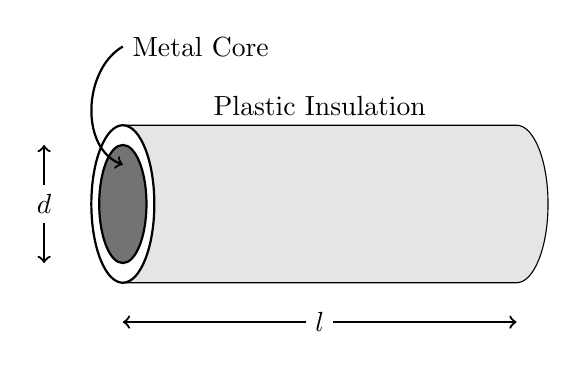
\begin{tikzpicture}
        %% Barrel
        \draw[fill=white!90!black] (0,1) -- (5,1) arc (90:-90:0.4cm and 1cm) -- (0,-1) arc(270:90:0.4cm and 1cm) --cycle;
        \draw[thick,fill=white] (0,0) circle (0.4cm and 1cm);
        \draw[thick,fill=white!45!black] (0,0) circle (0.3cm and 0.75cm);
        %% Labels
        \node[anchor=south] at (2.5,1) {Plastic Insulation};
        \node[anchor=west] (M) at (0,2) {Metal Core};
        \draw[thick,<-] (0,0.5) to[out=160,in=210] (M.west);
        %% Labels
        \draw[thick,<->] (0,-1.5) -- (5,-1.5) node[pos=0.5,anchor=center,fill=white] {$l$};
        \draw[thick,<->] (-1,0.75) -- (-1,-0.75) node[pos=0.5,anchor=center,fill=white] {$d$};
    \end{tikzpicture}
    \end{center}
    A decrease in the resistance of the wire would be produced by an increase in the:
    \begin{choices}
        \wrongchoice{thickness of the plastic insulation}
        \wrongchoice{length $l$ of the wire}
      \correctchoice{diameter $d$ of the wire}
        \wrongchoice{temperature of the wire}
    \end{choices}
\end{question}
}

\element{nysed}{
\begin{question}{June2001-Q31}
    A current of \SI{3.0}{\ampere} is flowing in a circuit.
    How much charge passes a given point in the circuit in \SI{30}{\second}?
    \begin{multicols}{2}
    \begin{choices}
        \wrongchoice{\SI{0.10}{\coulomb}}
        \wrongchoice{\SI{10}{\coulomb}}
        \wrongchoice{\SI{33}{\coulomb}}
      \correctchoice{\SI{90}{\coulomb}}
    \end{choices}
    \end{multicols}
\end{question}
}


%% Section Jan2001
%%--------------------
\element{nysed}{
\begin{question}{Jan2001-Q26}
    Compared to insulators, metals are better conductors of electricity because metals contain more free:
    \begin{multicols}{2}
    \begin{choices}
        \wrongchoice{protons}
      \correctchoice{electrons}
        \wrongchoice{positive ions}
        \wrongchoice{negative ions}
    \end{choices}
    \end{multicols}
\end{question}
}

\element{nysed}{
\begin{question}{Jan2001-Q29}
    A metal wire has length $L$ and cross-sectional area $A$.
    The resistance of the wire is directly proportional to:
    \begin{multicols}{2}
    \begin{choices}
      \correctchoice{$\dfrac{L}{A}$}
        \wrongchoice{$L \times A$}
        \wrongchoice{$\dfrac{A}{L}$}
        \wrongchoice{$L + A$}
    \end{choices}
    \end{multicols}
\end{question}
}

\element{nysed}{
\begin{question}{Jan2001-Q35}
    A wire carries a current of \SI{2.0}{\ampere}.
    How many electrons pass a given point in this wire in \SI{1.0}{\second}?
    \begin{multicols}{2}
    \begin{choices}
        \wrongchoice{\num{1.3e18}}
        \wrongchoice{\num{2.0e18}}
      \correctchoice{\num{1.3e19}}
        \wrongchoice{\num{2.0e19}}
    \end{choices}
    \end{multicols}
\end{question}
}


%% Section June2000
%%--------------------
\element{nysed}{
\begin{question}{June2000-Q26}
    A lightning bolt transfers \SI{6.0}{\coulomb} of charge from a cloud to the ground in \SI{2.0e-3}{\second}.
    What is the average current during this event?
    \begin{multicols}{2}
    \begin{choices}
        \wrongchoice{\SI{1.2e-2}{\ampere}}
        \wrongchoice{\SI{3.0e2}{\ampere}}
      \correctchoice{\SI{3.0e3}{\ampere}}
        \wrongchoice{\SI{1.2e4}{\ampere}}
    \end{choices}
    \end{multicols}
\end{question}
}

\element{nysed}{
\begin{question}{June2000-Q27}
    Conductivity in metallic solids is due to the presence of free:
    \begin{multicols}{2}
    \begin{choices}
        \wrongchoice{nuclei}
        \wrongchoice{protons}
        \wrongchoice{neutrons}
      \correctchoice{electrons}
    \end{choices}
    \end{multicols}
\end{question}
}

\element{nysed}{
\begin{question}{June2000-Q32}
    The graph below represents the relationship between the potential difference across a metal conductor and the current through the conductor at a constant temperature.
    \begin{center}
    \begin{tikzpicture}
        \begin{axis}[
            axis y line=left,
            axis x line=bottom,
            axis line style={->},
            ylabel={potential},
            y unit=\si{\volt},
            ytick={0,2.0,4.0,6.0,8.0},
            xlabel={current},
            x unit=\si{\ampere},
            xtick={0,0.2,0.4,0.6,0.8},
            xmin=0,xmax=0.9,
            ymin=0,ymax=8,
            grid=major,
            width=0.8\columnwidth,
            height=0.5\columnwidth,
            very thin,
        ]
        \addplot[line width=1pt,domain=0:0.9]{10*x};
        \end{axis}
    \end{tikzpicture}
    \end{center}
    What is the resistance of the conductor?
    \begin{multicols}{2}
    \begin{choices}
        \wrongchoice{\SI{1}{\ohm}}
        \wrongchoice{\SI{0.01}{\ohm}}
        \wrongchoice{\SI{0.1}{\ohm}}
      \correctchoice{\SI{10}{\ohm}}
    \end{choices}
    \end{multicols}
\end{question}
}

\element{nysed}{
\begin{question}{June2000-Q40}
    The heating element on an electric stove dissipates \SI{4.0e2}{\watt} of power when connected to a \SI{120}{\volt} source.
    What is the electrical resistance of this heating element?
    \begin{multicols}{2}
    \begin{choices}
        \wrongchoice{\SI{0.028}{\ohm}}
        \wrongchoice{\SI{0.60}{\ohm}}
        \wrongchoice{\SI{3.3}{\ohm}}
      \correctchoice{\SI{36}{\ohm}}
    \end{choices}
    \end{multicols}
\end{question}
}

\element{nysed}{
\begin{question}{June2000-Q77}
    A simple electrical circuit contains a battery,
        a light bulb, and a properly connected ammeter.
    The ammeter has a very low internal resistance because it is connect in:
    \begin{choices}
        \wrongchoice{parallel with the bulb to have little effect on the current through the bulb}
        \wrongchoice{parallel with the bulb to prevent current flow through the bulb}
      \correctchoice{series with the bulb to have little effect on the current through the bulb}
        \wrongchoice{series with the bulb to prevent current flow through the bulb}
    \end{choices}
\end{question}
}


%% Section June1999
%%--------------------
\element{nysed}{
\begin{question}{June1999-Q31}
    A metallic conductor obeys Ohm's law.
    Which graph best represents the relationship between the potential difference across the conductor and the resulting current through the conductor?
    \begin{multicols}{2}
    \begin{choices}
        \AMCboxDimensions{down=-2.5em}
        \correctchoice{
            \begin{tikzpicture}
                \begin{axis}[
                    axis y line=left,
                    axis x line=bottom,
                    axis line style={->},
                    ylabel={potential},
                    ytick=\empty,
                    xlabel={current},
                    xtick=\empty,
                    xmin=0,xmax=11,
                    ymin=0,ymax=11,
                    width=\columnwidth,
                    very thin,
                ]
                \addplot[line width=1pt,domain=0:10]{x};
                \end{axis}
            \end{tikzpicture}
        }
        \wrongchoice{
            \begin{tikzpicture}
                \begin{axis}[
                    axis y line=left,
                    axis x line=bottom,
                    axis line style={->},
                    ylabel={potential},
                    ytick=\empty,
                    xlabel={current},
                    xtick=\empty,
                    xmin=0,xmax=11,
                    ymin=0,ymax=11,
                    width=\columnwidth,
                    very thin,
                ]
                \addplot[line width=1pt,domain=0:10]{5};
                \end{axis}
            \end{tikzpicture}
        }
        \wrongchoice{
            \begin{tikzpicture}
                \begin{axis}[
                    axis y line=left,
                    axis x line=bottom,
                    axis line style={->},
                    ylabel={potential},
                    ytick=\empty,
                    xlabel={current},
                    xtick=\empty,
                    xmin=0,xmax=11,
                    ymin=0,ymax=11,
                    width=\columnwidth,
                    very thin,
                ]
                \addplot[line width=1pt,domain=0:10]{10-x};
                \end{axis}
            \end{tikzpicture}
        }
        \wrongchoice{
            \begin{tikzpicture}
                \begin{axis}[
                    axis y line=left,
                    axis x line=bottom,
                    axis line style={->},
                    ylabel={potential},
                    ytick=\empty,
                    xlabel={current},
                    xtick=\empty,
                    xmin=0,xmax=11,
                    ymin=0,ymax=11,
                    width=\columnwidth,
                    very thin,
                ]
                \addplot[line width=1pt,domain=0:10]{10/x};
                \end{axis}
            \end{tikzpicture}
        }
    \end{choices}
    \end{multicols}
\end{question}
}

\element{nysed}{
\begin{question}{June1999-Q32}
    A light bulb operating at \SI{120}{\volt} draws a current of \SI{0.50}{\ampere} for \SI{240}{\second}.
    The power rating of the light bulb is:
    \begin{multicols}{2}
    \begin{choices}
        \wrongchoice{\SI{30}{\watt}}
      \correctchoice{\SI{60}{\watt}}
        \wrongchoice{\SI{75}{\watt}}
        \wrongchoice{\SI{120}{\watt}}
    \end{choices}
    \end{multicols}
\end{question}
}

\element{nysed}{
\begin{question}{June1999-Q37}
    %The table below shows the length and cross-sectional area of four pieces of copper wire at the same temperature.
    Four pieces of copper wire at the same temperature are described below.
    Which wire has the highest resistance?
    \begin{center}
    \begin{tabu}{cX[c]X[2c]}
        \toprule
        \makebox[1.5em][c]{\textnumero}
            & Length [\si{\meter}] & Cross-Sectional Area [\si{\meter\squared}] \\
        \bottomrule
    \end{tabu}
    \end{center}
    \begin{choices}
        \wrongchoice{\begin{tabu}{X[c]X[2c]} 10 & \num{2e-6} \\ \end{tabu}}
      \correctchoice{\begin{tabu}{X[c]X[2c]} 10 & \num{1e-6} \\ \end{tabu}}
        \wrongchoice{\begin{tabu}{X[c]X[2c]} 1 & \num{2e-6} \\ \end{tabu}}
        \wrongchoice{\begin{tabu}{X[c]X[2c]} 1 & \num{1e-6} \\ \end{tabu}}
    \end{choices}
\end{question}
}

\element{nysed}{
\begin{question}{June1999-Q76}
    Which graph best represents the relationship between the deflection of a galvanometer coil and the current passing through the coil?
    \begin{multicols}{2}
    \begin{choices}
        \AMCboxDimensions{down=-2.5em}
        \correctchoice{
            \begin{tikzpicture}
                \begin{axis}[
                    axis y line=left,
                    axis x line=bottom,
                    axis line style={->},
                    ylabel={deflection},
                    ytick=\empty,
                    xlabel={current},
                    xtick=\empty,
                    xmin=0,xmax=11,
                    ymin=0,ymax=11,
                    width=\columnwidth,
                    very thin,
                ]
                \addplot[line width=1pt,domain=0:10]{x};
                \end{axis}
            \end{tikzpicture}
        }
        \wrongchoice{
            \begin{tikzpicture}
                \begin{axis}[
                    axis y line=left,
                    axis x line=bottom,
                    axis line style={->},
                    ylabel={deflection},
                    ytick=\empty,
                    xlabel={current},
                    xtick=\empty,
                    xmin=0,xmax=11,
                    ymin=0,ymax=11,
                    width=\columnwidth,
                    very thin,
                ]
                \addplot[line width=1pt,domain=0:10]{0.1*x^2};
                \end{axis}
            \end{tikzpicture}
        }
        \wrongchoice{
            \begin{tikzpicture}
                \begin{axis}[
                    axis y line=left,
                    axis x line=bottom,
                    axis line style={->},
                    ylabel={deflection},
                    ytick=\empty,
                    xlabel={current},
                    xtick=\empty,
                    xmin=0,xmax=11,
                    ymin=0,ymax=11,
                    width=\columnwidth,
                    very thin,
                ]
                \addplot[line width=1pt,domain=0:10]{10/x};
                \end{axis}
            \end{tikzpicture}
        }
        \wrongchoice{
            \begin{tikzpicture}
                \begin{axis}[
                    axis y line=left,
                    axis x line=bottom,
                    axis line style={->},
                    ylabel={deflection},
                    ytick=\empty,
                    xlabel={current},
                    xtick=\empty,
                    xmin=0,xmax=11,
                    ymin=0,ymax=11,
                    width=\columnwidth,
                    very thin,
                ]
                \addplot[line width=1pt,domain=0:10]{8};
                \end{axis}
            \end{tikzpicture}
        }
    \end{choices}
    \end{multicols}
\end{question}
}



%% Section June1998
%%--------------------
\element{nysed}{
\begin{question}{June1998-Q27}
    What is the potential difference across a \SI{2.0}{\ohm} resistor that draws \SI{2.0}{\coulomb\per\second}?
    \begin{multicols}{2}
    \begin{choices}
        \wrongchoice{\SI{1.0}{\volt}}
        \wrongchoice{\SI{2.0}{\volt}}
        \wrongchoice{\SI{3.0}{\volt}}
      \correctchoice{\SI{4.0}{\volt}}
    \end{choices}
    \end{multicols}
\end{question}
}

\element{nysed}{
\begin{question}{June1998-Q30}
    An electric motor draws \SI{150}{\ampere} of current while operating at \SI{240}{\volt}.
    What is the power rating of this motor?
    \begin{multicols}{2}
    \begin{choices}
        \wrongchoice{\SI{1.6}{\watt}}
        \wrongchoice{\SI{3.8e2}{\watt}}
      \correctchoice{\SI{3.6e4}{\watt}}
        \wrongchoice{\SI{5.4e6}{\watt}}
    \end{choices}
    \end{multicols}
\end{question}
}

\element{nysed}{
\begin{question}{June1998-Q31}
    An operating \SI{75}{\watt} lamp is connected to a \SI{120}{\volt} outlet.
    How much electrical energy is used by the lamp in \SI{60}{\minute} (\SI{3600}{\second})?
    \begin{multicols}{2}
    \begin{choices}
        \wrongchoice{\SI{4.5e3}{\joule}}
      \correctchoice{\SI{2.7e5}{\joule}}
        \wrongchoice{\SI{5.4e5}{\joule}}
        \wrongchoice{\SI{3.2e7}{\joule}}
    \end{choices}
    \end{multicols}
\end{question}
}



%% Section June1997
%%--------------------
\element{nysed}{
\begin{question}{June1997-Q28}
    An operating lamp draws a current of \SI{0.5}{\ampere}.
    The amount of charge passing through the lamp in \SI{10}{\second} is:
    \begin{multicols}{2}
    \begin{choices}
        \wrongchoice{\SI{0.050}{\coulomb}}
        \wrongchoice{\SI{2.0}{\coulomb}}
      \correctchoice{\SI{5.0}{\coulomb}}
        \wrongchoice{\SI{20}{\coulomb}}
    \end{choices}
    \end{multicols}
\end{question}
}

\element{nysed}{
\begin{question}{June1997-Q29}
    Which graph best represents the relationship between the resistance of a copper wire of uniform cross-sectional area and the wire's length at constant temperature?
    \begin{multicols}{2}
    \begin{choices}
        \AMCboxDimensions{down=-2.5em}
        \correctchoice{
            \begin{tikzpicture}
                \begin{axis}[
                    axis y line=left,
                    axis x line=bottom,
                    axis line style={->},
                    ylabel={resistance},
                    ytick=\empty,
                    xlabel={length},
                    xtick=\empty,
                    xmin=0,xmax=11,
                    ymin=0,ymax=11,
                    width=\columnwidth,
                    very thin,
                ]
                \addplot[line width=1pt,domain=0:10]{x};
                \end{axis}
            \end{tikzpicture}
        }
        \wrongchoice{
            \begin{tikzpicture}
                \begin{axis}[
                    axis y line=left,
                    axis x line=bottom,
                    axis line style={->},
                    ylabel={resistance},
                    ytick=\empty,
                    xlabel={length},
                    xtick=\empty,
                    xmin=0,xmax=11,
                    ymin=0,ymax=11,
                    width=\columnwidth,
                    very thin,
                ]
                \addplot[line width=1pt,domain=0:10]{5};
                \end{axis}
            \end{tikzpicture}
        }
        \wrongchoice{
            \begin{tikzpicture}
                \begin{axis}[
                    axis y line=left,
                    axis x line=bottom,
                    axis line style={->},
                    ylabel={resistance},
                    ytick=\empty,
                    xlabel={length},
                    xtick=\empty,
                    xmin=0,xmax=11,
                    ymin=0,ymax=11,
                    width=\columnwidth,
                    very thin,
                ]
                \addplot[line width=1pt,domain=0:10]{10-x};
                \end{axis}
            \end{tikzpicture}
        }
        \wrongchoice{
            \begin{tikzpicture}
                \begin{axis}[
                    axis y line=left,
                    axis x line=bottom,
                    axis line style={->},
                    ylabel={resistance},
                    ytick=\empty,
                    xlabel={length},
                    xtick=\empty,
                    xmin=0,xmax=11,
                    ymin=0,ymax=11,
                    width=\columnwidth,
                    very thin,
                ]
                \addplot[line width=1pt,domain=0:10]{10/x};
                \end{axis}
            \end{tikzpicture}
        }
    \end{choices}
    \end{multicols}
\end{question}
}


\element{nysed}{
\begin{question}{June1997-Q31}
    To increase the brightness of a desk lamp,
        a student replaces a \SI{60}{\watt} light bulb with a \SI{100}{\watt} light bulb.
    Compared to the \SI{60}{\watt} bulb,
        the \SI{100}{\watt} bulb has:
    \begin{choices}
      \correctchoice{less resistance and draws more current.}
        \wrongchoice{less resistance and draws less current.}
        \wrongchoice{more resistance and draws more current.}
        \wrongchoice{more resistance and draws less current.}
    \end{choices}
\end{question}
}

\element{nysed}{
\begin{question}{June1997-Q32}
    An electric dryer consumed \SI{6.0e6}{\joule} of energy when operating at \SI{220}{\volt} for \SI{30}{\minute} (\SI{1800}{\second}).
    During operation, the dryer draws a current of approximately:
    \begin{multicols}{2}
    \begin{choices}
        \wrongchoice{\SI{10}{\ampere}}
      \correctchoice{\SI{15}{\ampere}}
        \wrongchoice{\SI{20}{\ampere}}
        \wrongchoice{\SI{25}{\ampere}}
    \end{choices}
    \end{multicols}
\end{question}
}



%% Section June1996
%%--------------------
\element{nysed}{
\begin{question}{June1996-Q29}
    A metal conductor is used in an electric circuit.
    The electrical resistance provided by the conductor could be increase by:
    \begin{choices}
        \wrongchoice{decreasing the length of the conductor.}
        \wrongchoice{decreasing the applied voltage in the circuit.}
      \correctchoice{increasing the temperature of the conductor.}
        \wrongchoice{increasing the cross-sectional area of the conductor.}
    \end{choices}
\end{question}
}

\element{nysed}{
\begin{question}{June1996-Q31}
    In a lightning strike,
        a charge of \SI{18}{\coulomb} is transferred between a cloud and the ground in \SI{2.0e-2}{\second} at a potential difference of \SI{1.5e6}{\volt}.
    What is the average current produced by this strike?
    \begin{multicols}{2}
    \begin{choices}
        \wrongchoice{\SI{3.6e-1}{\ampere}}
      \correctchoice{\SI{9.0e2}{\ampere}}
        \wrongchoice{\SI{3.0e4}{\ampere}}
        \wrongchoice{\SI{7.5e7}{\ampere}}
    \end{choices}
    \end{multicols}
\end{question}
}

\element{nysed}{
\begin{question}{June1996-Q36}
    If the potential drop across an operating \SI{300}{\watt} flood-light is \SI{120}{\volt},
        what is the current through the floodlight?
    \begin{multicols}{2}
    \begin{choices}
        \wrongchoice{\SI{0.40}{\ampere}}
      \correctchoice{\SI{2.5}{\ampere}}
        \wrongchoice{\SI{7.5}{\ampere}}
        \wrongchoice{\SI{4.8}{\ampere}}
    \end{choices}
    \end{multicols}
\end{question}
}


%% Section June1995
%%--------------------
\element{nysed}{
\begin{question}{June1995-Q26}
    A \SI{20}{\ohm} resistor has \SI{40}{\coulomb} passing through it in \SI{5.0}{\second}.
    The potential difference across the resistor is:
    \begin{multicols}{2}
    \begin{choices}
        \wrongchoice{\SI{8.0}{\volt}}
        \wrongchoice{\SI{100}{\volt}}
      \correctchoice{\SI{160}{\volt}}
        \wrongchoice{\SI{200}{\volt}}
    \end{choices}
    \end{multicols}
\end{question}
}

\element{nysed}{
\begin{question}{June1995-Q27}
    The diagram below shows a circuit in which a copper wire connects points $A$ and $B$.
    \begin{center}
    \ctikzset{bipoles/length=1.00cm}
    \begin{circuitikz}
        %% circuit
        \draw (4,0) to (2,0) to [R] (0,0) to (0,2) to [battery] (2,2) to (4,2) to (4,0);
        %% points A and B
        \fill (2.00,2) circle (1.5pt) node[anchor=south] {$A$};
        \fill (3.66,2) circle (1.5pt) node[anchor=south] {$B$};
    \end{circuitikz}
    \end{center}
    The electrical resistance between point $A$ and $B$ can be decreased by:
    \begin{choices}
      \correctchoice{replacing the wire with a thicker copper wire of the same length.}
        \wrongchoice{replacing the wire with a longer copper wire of the same thickness.}
        \wrongchoice{increasing the temperature of the copper wire.}
        \wrongchoice{increasing the potential difference supplied by the battery.}
    \end{choices}
\end{question}
}

\element{nysed}{
\begin{question}{June1995-Q29}
    Which unit is equivalent to a watt, the SI unit of power?
    \begin{choices}
      \correctchoice{joule per second (\si{\joule\per\second})}
        \wrongchoice{joule per volt (\si{\joule\per\volt})}
        \wrongchoice{joule per ohm (\si{\joule\per\ohm})}
        \wrongchoice{joule per coulomb (\si{\joule\per\coulomb})}
    \end{choices}
\end{question}
}

\element{nysed}{
\begin{question}{June1995-Q30}
    An electric fan draws \SI{1.7}{\ampere} of current when operated at a potential difference of \SI{120}{\volt}.
    How much electrical energy is needed to run this fan for 1 hour? [1 hour = 3600 seconds]
    \begin{multicols}{2}
    \begin{choices}
        \wrongchoice{\SI{7.1e1}{\joule}}
        \wrongchoice{\SI{2.0e2}{\joule}}
        \wrongchoice{\SI{2.5e5}{\joule}}
      \correctchoice{\SI{7.3e5}{\joule}}
    \end{choices}
    \end{multicols}
\end{question}
}


%% Section June1994
%%--------------------
\element{nysed}{
\begin{question}{June1994-Q29}
    A copper wire is connected across a constant voltage source.
    The current flowing in the wire can be increased by increasing the wire's:
    \begin{multicols}{2}
    \begin{choices}
      \correctchoice{cross-sectional area}
        \wrongchoice{length}
        \wrongchoice{resistance}
        \wrongchoice{temperature}
    \end{choices}
    \end{multicols}
\end{question}
}

\element{nysed}{
\begin{question}{June1994-Q31}
    A clothes dryer connected to a \SI{240}{\volt} line draws \SI{30}{\ampere} of current for \SI{20}{\minute} (\SI{1200}{\second}).
    Approximately how much electrical energy is consumed by the dryer?
    \begin{multicols}{2}
    \begin{choices}
        \wrongchoice{\SI{4.8e3}{\joule}}
        \wrongchoice{\SI{7.2e3}{\joule}}
        \wrongchoice{\SI{1.4e5}{\joule}}
      \correctchoice{\SI{8.6e6}{\joule}}
    \end{choices}
    \end{multicols}
\end{question}
}



%% Section June1990
%%--------------------
\element{nysed}{
\begin{question}{June1990-Q30}
    A copper wire has a resistance of \SI{200}{\ohm}.
    A second copper wire with twice the cross-sectional area and the same length would have a resistance of:
    \begin{multicols}{2}
    \begin{choices}
        \wrongchoice{\SI{50}{\ohm}}
      \correctchoice{\SI{100}{\ohm}}
        \wrongchoice{\SI{200}{\ohm}}
        \wrongchoice{\SI{400}{\ohm}}
    \end{choices}
    \end{multicols}
\end{question}
}

\element{nysed}{
\begin{question}{June1990-Q33}
    If 10 coulombs of charge passes a given point in a conductor every 2 seconds,
        the current at that point is:
    \begin{multicols}{2}
    \begin{choices}
        \wrongchoice{\SI{0.2}{\ampere}}
      \correctchoice{\SI{5}{\ampere}}
        \wrongchoice{\SI{10}{\ampere}}
        \wrongchoice{\SI{20}{\ampere}}
    \end{choices}
    \end{multicols}
\end{question}
}

\element{nysed}{
\begin{question}{June1990-Q34}
    The graph below shows the relationship between current and potential difference for four resistors, $A$, $B$, $C$, and $D$.
    \begin{center}
    \begin{tikzpicture}
        \begin{axis}[
            axis y line=left,
            axis x line=bottom,
            axis line style={->},
            xlabel={current},
            xtick=\empty,
            ylabel={potential},
            ytick=\empty,
            xmin=0,xmax=11,
            ymin=0,ymax=11,
            width=0.8\columnwidth,
            height=0.5\columnwidth,
            clip=false,
            very thin,
        ]
        \draw[thick] (axis cs:0,0) -- ++(80:10) node[anchor=south] {$A$};
        \draw[thick] (axis cs:0,0) -- ++(60:10) node[anchor=south] {$B$};
        \draw[thick] (axis cs:0,0) -- ++(40:10) node[anchor=south] {$C$};
        \draw[thick] (axis cs:0,0) -- ++(20:10) node[anchor=south] {$D$};
        \end{axis}
    \end{tikzpicture}
    \end{center}
    Which resistor has the greatest resistance?
    \begin{multicols}{4}
    \begin{choices}
      \correctchoice{$A$}
        \wrongchoice{$B$}
        \wrongchoice{$C$}
        \wrongchoice{$D$}
    \end{choices}
    \end{multicols}
\end{question}
}


%% Section June1989
%%--------------------
\element{nysed}{
\begin{question}{June1989-Q31}
    A charge of \SI{5.0}{\coulomb} moves through a circuit in \SI{0.50}{\second}.
    How much current is flowing through the circuit?
    \begin{multicols}{2}
    \begin{choices}
        \wrongchoice{\SI{2.5}{\ampere}}
        \wrongchoice{\SI{5.0}{\ampere}}
        \wrongchoice{\SI{7.0}{\ampere}}
      \correctchoice{\SI{10}{\ampere}}
    \end{choices}
    \end{multicols}
\end{question}
}

\element{nysed}{
\begin{question}{June1989-Q32}
    Which graph represents a circuit element at constant temperature that obeys Ohm's law?
    \begin{multicols}{2}
    \begin{choices}
        \AMCboxDimensions{down=-2.5em}
        \wrongchoice{
            \begin{tikzpicture}
                \begin{axis}[
                    axis y line=left,
                    axis x line=bottom,
                    axis line style={->},
                    xlabel={current},
                    xtick=\empty,
                    ylabel={voltage},
                    ytick=\empty,
                    xmin=0,xmax=11,
                    ymin=0,ymax=11,
                    width=\columnwidth,
                    very thin,
                ]
                \addplot[line width=1pt,domain=0:10]{8};
                \end{axis}
            \end{tikzpicture}
        }
        \wrongchoice{
            \begin{tikzpicture}
                \begin{axis}[
                    axis y line=left,
                    axis x line=bottom,
                    axis line style={->},
                    xlabel={current},
                    xtick=\empty,
                    ylabel={voltage},
                    ytick=\empty,
                    xmin=0,xmax=11,
                    ymin=0,ymax=11,
                    width=\columnwidth,
                    very thin,
                ]
                \addplot[line width=1pt,domain=0:10]{0.1*x*x};
                \end{axis}
            \end{tikzpicture}
        }
        \wrongchoice{
            \begin{tikzpicture}
                \begin{axis}[
                    axis y line=left,
                    axis x line=bottom,
                    axis line style={->},
                    xlabel={current},
                    xtick=\empty,
                    ylabel={voltage},
                    ytick=\empty,
                    xmin=0,xmax=11,
                    ymin=0,ymax=11,
                    width=\columnwidth,
                    very thin,
                ]
                \addplot[line width=1pt,domain=0:10]{10-x};
                \end{axis}
            \end{tikzpicture}
        }
        %% ANS is 4
        \correctchoice{
            \begin{tikzpicture}
                \begin{axis}[
                    axis y line=left,
                    axis x line=bottom,
                    axis line style={->},
                    xlabel={current},
                    xtick=\empty,
                    ylabel={voltage},
                    ytick=\empty,
                    xmin=0,xmax=11,
                    ymin=0,ymax=11,
                    width=\columnwidth,
                    very thin,
                ]
                \addplot[line width=1pt,domain=0:10]{x};
                \end{axis}
            \end{tikzpicture}
        }
    \end{choices}
    \end{multicols}
\end{question}
}


%% Section June1986
%%--------------------
\element{nysed}{
\begin{question}{June1986-Q38}
    A flow rate of \SI{1}{\coulomb} per \SI{0.1}{\second} is measured in a wire.
    What is the electrical current in the wire?
    \begin{multicols}{2}
    \begin{choices}
        \wrongchoice{\SI{1}{\ampere}}
        \wrongchoice{\SI{0.1}{\ampere}}
      \correctchoice{\SI{10}{\ampere}}
        \wrongchoice{\SI{100}{\ampere}}
    \end{choices}
    \end{multicols}
\end{question}
}

\element{nysed}{
\begin{question}{June1986-Q39}
    The graph at the right shows how the voltage and current are related in a simple electric circuit.
    \begin{center}
    \begin{tikzpicture}
        \begin{axis}[
            axis y line=left,
            axis x line=bottom,
            axis line style={->},
            xlabel={current},
            x unit=\si{\ampere},
            xtick=\empty,
            ylabel={voltage},
            y unit=\si{\volt},
            ytick=\empty,
            xmin=0,xmax=11,
            ymin=0,ymax=11,
            width=0.8\columnwidth,
            height=0.5\columnwidth,
            very thin,
        ]
        \addplot[line width=1pt,domain=0:10]{x};
        \end{axis}
    \end{tikzpicture}
    \end{center}
    For any point on the line,
        what does the ratio of $v$ to $I$ represent?
    \begin{choices}
        \wrongchoice{work in joules}
        \wrongchoice{power in watts}
      \correctchoice{resistance in ohms}
        \wrongchoice{charge in coulombs}
    \end{choices}
\end{question}
}

\element{nysed}{
\begin{question}{June1986-Q40}
    A \SI{10}{\volt} potential difference maintains a \SI{2}{\ampere} current in a resistor.
    The total energy expended by this resistor in \SI{5}{\second} is:
    \begin{multicols}{2}
    \begin{choices}
        \wrongchoice{\SI{10}{\joule}}
        \wrongchoice{\SI{20}{\joule}}
        \wrongchoice{\SI{50}{\joule}}
      \correctchoice{\SI{100}{\joule}}
    \end{choices}
    \end{multicols}
\end{question}
}

\element{nysed}{
\begin{question}{June1986-Q41}
    What is the current in ammeter $A$ in the diagram below?
    \begin{center}
    \ctikzset{bipoles/length=1.00cm}
    \begin{circuitikz}
        \draw (0,0) to [battery,l=\SI{9}{\volt}]
              (0,3) to (2,3) to [R,l=\SI{3}{\ohm}] (2,1.5) to (2,0) to (0,0);
        \draw (2,3) to (4,3) to [R,l=\SI{3}{\ohm}] (4,1.5) to [ammeter,l=$A$] (4,0) to (2,0);
        \draw (4,3) to (6,3) to [R,l=\SI{3}{\ohm}] (6,1.5) to (6,0) to (2,0);
    \end{circuitikz}
    \end{center}
    \begin{multicols}{4}
    \begin{choices}
        \wrongchoice{\SI{1}{\ampere}}
        \wrongchoice{\SI{1/3}{\ampere}}
      \correctchoice{\SI{3}{\ampere}}
        \wrongchoice{\SI{9}{\ampere}}
    \end{choices}
    \end{multicols}
\end{question}
}

\element{nysed}{
\begin{question}{June1986-Q59}
    The electrical resistance of a metal wire could be decreased by:
    \begin{choices}
        \wrongchoice{increasing its temperature}
      \correctchoice{increasing its diameter}
        \wrongchoice{increasing its length}
    \end{choices}
\end{question}
}


%% Section June1985
%%--------------------
\element{nysed}{
\begin{question}{June1985-Q35}
    Electrical conductivity in liquid solutions depends on the presence of free:
    \begin{multicols}{2}
    \begin{choices}
        \wrongchoice{neutrons}
        \wrongchoice{protons}
        \wrongchoice{molecules}
      \correctchoice{ions}
    \end{choices}
    \end{multicols}
\end{question}
}

\element{nysed}{
\begin{question}{June1985-Q39}
    Which graph best represents a material behaving according to Ohm's law?
    \begin{multicols}{2}
    \begin{choices}
        \AMCboxDimensions{down=-2.5em}
        %% ANS is 1
        \correctchoice{
            \begin{tikzpicture}
                \begin{axis}[
                    axis y line=left,
                    axis x line=bottom,
                    axis line style={->},
                    xlabel={potential},
                    x unit=\si{\volt},
                    xtick=\empty,
                    ylabel={current},
                    y unit=\si{\ampere},
                    ytick=\empty,
                    xmin=0,xmax=11,
                    ymin=0,ymax=11,
                    width=\columnwidth,
                    very thin,
                ]
                \addplot[line width=1pt,domain=0:10] {x};
                \end{axis}
            \end{tikzpicture}
        }
        \wrongchoice{
            \begin{tikzpicture}
                \begin{axis}[
                    axis y line=left,
                    axis x line=bottom,
                    axis line style={->},
                    xlabel={potential},
                    x unit=\si{\volt},
                    xtick=\empty,
                    ylabel={current},
                    y unit=\si{\ampere},
                    ytick=\empty,
                    xmin=0,xmax=11,
                    ymin=0,ymax=11,
                    width=\columnwidth,
                    very thin,
                ]
                \addplot[line width=1pt,domain=0:10] {sqrt(10)*sqrt(x)};
                \end{axis}
            \end{tikzpicture}
        }
        \wrongchoice{
            \begin{tikzpicture}
                \begin{axis}[
                    axis y line=left,
                    axis x line=bottom,
                    axis line style={->},
                    xlabel={potential},
                    x unit=\si{\volt},
                    xtick=\empty,
                    ylabel={current},
                    y unit=\si{\ampere},
                    ytick=\empty,
                    xmin=0,xmax=11,
                    ymin=0,ymax=11,
                    width=\columnwidth,
                    very thin,
                ]
                \addplot[line width=1pt,domain=0:10] {10-x};
                \end{axis}
            \end{tikzpicture}
        }
        \wrongchoice{
            \begin{tikzpicture}
                \begin{axis}[
                    axis y line=left,
                    axis x line=bottom,
                    axis line style={->},
                    xlabel={potential},
                    x unit=\si{\volt},
                    xtick=\empty,
                    ylabel={current},
                    y unit=\si{\ampere},
                    ytick=\empty,
                    xmin=0,xmax=11,
                    ymin=0,ymax=11,
                    width=\columnwidth,
                    very thin,
                ]
                \addplot[line width=1pt,domain=0:10] {10/x};
                \end{axis}
            \end{tikzpicture}
        }
    \end{choices}
    \end{multicols}
\end{question}
}

\element{nysed}{
\begin{question}{June1985-Q58}
    As the temperature of a metallic conductor increases,
        its resistance usually:
    \begin{choices}
        \wrongchoice{decreases}
      \correctchoice{increases}
        \wrongchoice{remains the same}
    \end{choices}
\end{question}
}

\element{nysed}{
\begin{question}{June1985-Q97}
    An electric heater rated at \SI{4 800}{\watt} is operated on \SI{120}{\volt}.
    %% start question
    What is the resistance of the heater?
    \begin{multicols}{2}
    \begin{choices}
        \wrongchoice{\SI{576 000}{\ohm}}
        \wrongchoice{\SI{120}{\ohm}}
      \correctchoice{\SI{3.0}{\ohm}}
        \wrongchoice{\SI{40}{\ohm}}
    \end{choices}
    \end{multicols}
\end{question}
}

\element{nysed}{
\begin{question}{June1985-Q98}
    An electric heater rated at \SI{4 800}{\watt} is operated on \SI{120}{\volt}.
    %% start question
    How much energy is used by this heater in \SI{10.0}{\second}?
    \begin{multicols}{2}
    \begin{choices}
        \wrongchoice{\SI{1.15}{\joule}}
        \wrongchoice{\SI{40}{\joule}}
        \wrongchoice{\SI{4.8e3}{\joule}}
      \correctchoice{\SI{4.8e4}{\joule}}
    \end{choices}
    \end{multicols}
\end{question}
}

\element{nysed}{
\begin{question}{June1985-Q99}
    An electric heater rated at \SI{4 800}{\watt} is operated on \SI{120}{\volt}.
    %% start question
    If the heater were replaced by one having a greater resistance,
        the amount of heat produced each second would:
    \begin{choices}
      \correctchoice{decrease}
        \wrongchoice{increase}
        \wrongchoice{remain the same}
    \end{choices}
\end{question}
}

\element{nysed}{
\begin{question}{June1985-Q101}
    An electric heater rated at \SI{4 800}{\watt} is operated on \SI{120}{\volt}.
    %% start question
    If the original heater were operated at less than \SI{120}{\volt},
        the amount of heat produced would:
    \begin{choices}
        \wrongchoice{decrease}
      \correctchoice{increase}
        \wrongchoice{remain the same}
    \end{choices}
\end{question}
}


\endinput


